\documentclass[ucs,9pt]{beamer}

% Copyright 2004 by Till Tantau <tantau@users.sourceforge.net>.
%
% In principle, this file can be redistributed and/or modified under
% the terms of the GNU Public License, version 2.
%
% However, this file is supposed to be a template to be modified
% for your own needs. For this reason, if you use this file as a
% template and not specifically distribute it as part of a another
% package/program, I grant the extra permission to freely copy and
% modify this file as you see fit and even to delete this copyright
% notice.
%
% Modified by Tobias G. Pfeiffer <tobias.pfeiffer@math.fu-berlin.de>
% to show usage of some features specific to the FU Berlin template.

% remove this line and the "ucs" option to the documentclass when your editor is not utf8-capable
\usepackage[utf8x]{inputenc}    % to make utf-8 input possible
\usepackage[english]{babel}     % hyphenation etc., alternatively use 'german' as 
\usepackage{tikz}
% Template for talks using the Corporate Design of the Freie Universitaet
%   Berlin, created following the guidelines on www.fu-berlin.de/cd by
%   Tobias G. Pfeiffer, <tobias.pfeiffer@math.fu-berlin.de>
% This file can be redistributed and/or modified in any way you like.
%   If you feel you have done significant improvements to this template,
%   please consider providing your modified version to
%   https://www.mi.fu-berlin.de/w/Mi/BeamerTemplateCorporateDesign

\usepackage{amsmath,dsfont,listings}

%%% FU logo
% small version for upper right corner of normal pages
\pgfdeclareimage[height=1.4cm]{university-logo}{gw_logo.eps}
\logo{\pgfuseimage{university-logo}}
% large version for upper right corner of title page
\pgfdeclareimage[height=1.4cm]{big-university-logo}{gw_logo.eps}
\newcommand{\titleimage}[1]{\pgfdeclareimage[height=2.92cm]{title-image}{#1}}
\titlegraphic{\pgfuseimage{title-image}}
%%% end FU logo

% NOTE: 1cm = 0.393 in = 28.346 pt;    1 pt = 1/72 in = 0.0352 cm
\setbeamersize{text margin right=3.5mm, text margin left=7.5mm}  % text margin

% colors to be used
\definecolor{text-grey}{rgb}{0.45, 0.45, 0.45} % grey text on white background
\definecolor{bg-grey}{rgb}{0.66, 0.65, 0.60} % grey background (for white text)
\definecolor{fu-blue}{RGB}{0, 51, 102} % blue text
\definecolor{fu-green}{RGB}{153, 204, 0} % green text
\definecolor{fu-red}{RGB}{204, 0, 0} % red text (used by \alert)

% switch off the sidebars
% TODO: loading \useoutertheme{sidebar} (which is maybe wanted) also inserts
%   a sidebar on title page (unwanted), also indents the page title (unwanted?),
%   and duplicates the navigation symbols (unwanted)
\setbeamersize{sidebar width left=0cm, sidebar width right=0mm}
\setbeamertemplate{sidebar right}{}
\setbeamertemplate{sidebar left}{}
%    XOR
% \useoutertheme{sidebar}

% frame title
% is truncated before logo and splits on two lines
% if neccessary (or manually using \\)
\setbeamertemplate{frametitle}{%
    \vskip-30pt \color{text-grey}\large%
    \begin{minipage}[b][23pt]{80.5mm}%
    \flushleft\insertframetitle%
    \end{minipage}%
}

%%% title page
% TODO: get rid of the navigation symbols on the title page.
%   actually, \frame[plain] *should* remove them...
\setbeamertemplate{title page}{
% upper right: FU logo
\vskip2pt\hfill\pgfuseimage{big-university-logo} \\
\vskip6pt\hskip3pt
% title image of the presentation
\begin{minipage}{11.6cm}
\hspace{-1mm}\inserttitlegraphic
\end{minipage}

% set the title and the author
\vskip14pt
\parbox[top][1.35cm][c]{11cm}{\color{text-grey}\inserttitle \\ \small \insertsubtitle}
\vskip11pt
\parbox[top][1.35cm][c]{11cm}{\small \insertauthor \\ \insertinstitute \\[3mm] \insertdate}
}
%%% end title page

%%% colors
\usecolortheme{lily}
\setbeamercolor*{normal text}{fg=black,bg=white}
\setbeamercolor*{alerted text}{fg=fu-red}
\setbeamercolor*{example text}{fg=fu-green}
\setbeamercolor*{structure}{fg=fu-blue}

\setbeamercolor*{block title}{fg=white,bg=black!50}
\setbeamercolor*{block title alerted}{fg=white,bg=black!50}
\setbeamercolor*{block title example}{fg=white,bg=black!50}

\setbeamercolor*{block body}{bg=black!10}
\setbeamercolor*{block body alerted}{bg=black!10}
\setbeamercolor*{block body example}{bg=black!10}

\setbeamercolor{bibliography entry author}{fg=fu-blue}
% TODO: this doesn't work at all:
\setbeamercolor{bibliography entry journal}{fg=text-grey}

\setbeamercolor{item}{fg=fu-blue}
\setbeamercolor{navigation symbols}{fg=text-grey,bg=bg-grey}
%%% end colors

%%% headline
\setbeamertemplate{headline}{
\vskip4pt\hfill\insertlogo\hspace{3.5mm} % logo on the right

\vskip6pt\color{fu-blue}\rule{\textwidth}{0.4pt} % horizontal line
}
%%% end headline

%%% footline
\newcommand{\footlinetext}{\insertshortinstitute, \insertshorttitle, \insertshortdate}
\setbeamertemplate{footline}{
\vskip5pt\color{fu-blue}\rule{\textwidth}{0.4pt}\\ % horizontal line
\vskip2pt
\makebox[123mm]{\hspace{7.5mm}
\color{fu-blue}\footlinetext
\hfill \raisebox{-1pt}{\usebeamertemplate***{navigation symbols}}
\hfill \insertframenumber}
\vskip4pt
}
%%% end footline

%%% settings for listings package
\lstset{extendedchars=true, showstringspaces=false, basicstyle=\footnotesize\sffamily, tabsize=2, breaklines=true, breakindent=10pt, frame=l, columns=fullflexible}
\lstset{language=Java} % this sets the syntax highlighting
\lstset{mathescape=true} % this switches on $...$ substitution in code
% enables UTF-8 in source code:
\lstset{literate={ä}{{\"a}}1 {ö}{{\"o}}1 {ü}{{\"u}}1 {Ä}{{\"A}}1 {Ö}{{\"O}}1 {Ü}{{\"U}}1 {ß}{\ss}1}
%%% end listings  % THIS is the line that includes the FU template!
\usepackage{amsmath}
\newcommand{\deriv}[2]{\frac{\mathrm{d}#1}{\mathrm{d}#2}}
%%\usepackage{breqn}
\newcommand{\pderiv}[2]{\frac{\partial#1}{\partial#2}}
\usepackage{arev,t1enc} % looks nicer than the standard sans-serif font
% if you experience problems, comment out the line above and change
% the documentclass option "9pt" to "10pt"

% image to be shown on the title page (without file extension, should be pdf or png)
\titleimage{bank} %use the jpeg neworleans file because it fits better

\title[Cost-Shifting] % (optional, use only with long paper titles)
{Hospital Pricing and Public Payments}

\subtitle
{}

\author[Author] % (optional, use only with lots of authors)
{Michael Darden, Ian McCarthy, and Eric Barrette}
% - Give the names in the same order as the appear in the paper.

\institute[George Washington University] % (optional, but mostly needed)
{}
% - Keep it simple, no one is interested in your street address.

\date[3/1/2018] % (optional, should be abbreviation of conference name)
{March 1st, 2018}
% - Either use conference name or its abbreviation.
% - Not really informative to the audience, more for people (including
%   yourself) who are reading the slides online

\subject{}
% This is only inserted into the PDF information catalog. Can be left
% out.

% you can redefine the text shown in the footline. use a combination of
% \insertshortauthor, \insertshortinstitute, \insertshorttitle, \insertshortdate, ...


% Delete this, if you do not want the table of contents to pop up at
% the beginning of each subsection:
\AtBeginSubsection[]
{
  \begin{frame}<beamer>{Outline}
    \tableofcontents[currentsection,currentsubsection]
  \end{frame}
}
\begin{document}

\begin{frame}[plain]
  \titlepage
\end{frame}

\begin{frame}{Outline}
  \tableofcontents
  % You might wish to add the option [pausesections]
\end{frame}
\begin{frame}
\frametitle{Health Care and Hospitals}
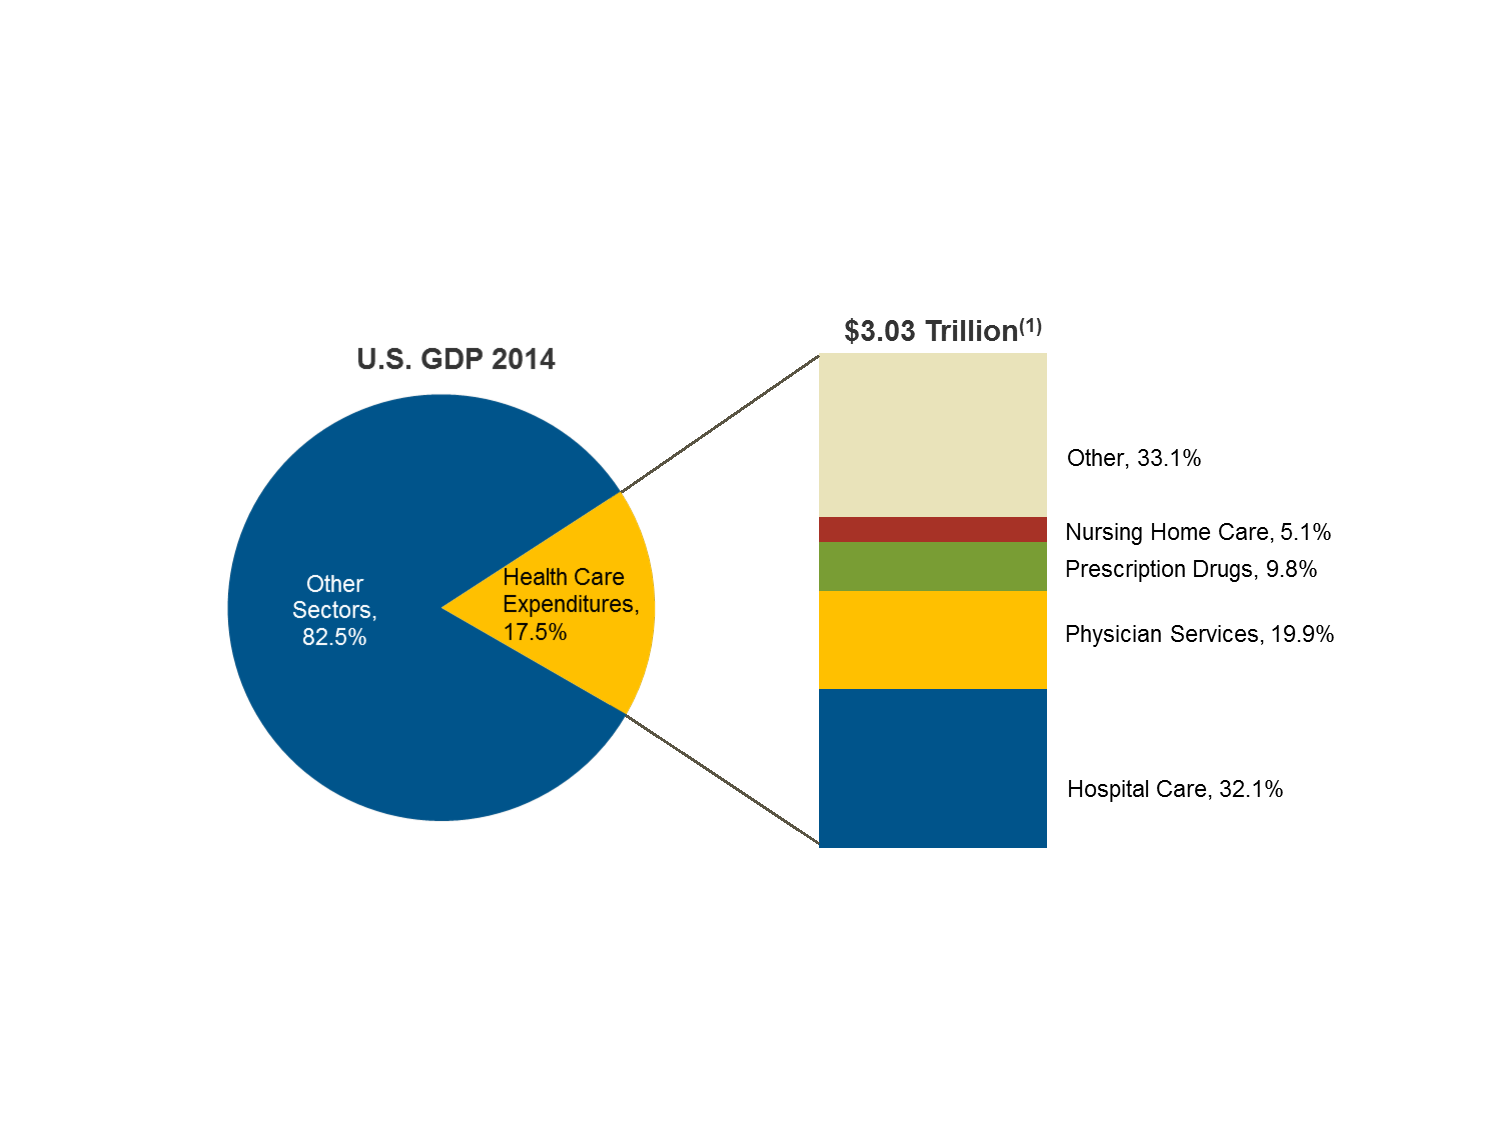
\includegraphics[scale=0.62]{6_1}
\end{frame}
\section{Introduction}






%\begin{frame}{The Questions We Answer}
%\begin{enumerate}
%\item {\bf Do hospitals respond to public reimbursement cuts by bargaining for higher prices from private insurers?  Do hospitals \textcolor{red}{cost-shift}? }
%\pause
%\item {\bf What characteristics of hospitals are associated with \textcolor{red}{cost-shifting?}}
%\item {\bf Can we rationalize cost-shifting behavior in the modern health care environment for both non-profit and for-profit hospitals?}
%\end{enumerate}
%\end{frame}





\subsection{Evidence in Favor of Cost-Shifting}


\begin{frame}
\frametitle{Hospital Cost-Shifting}
\begin{center}
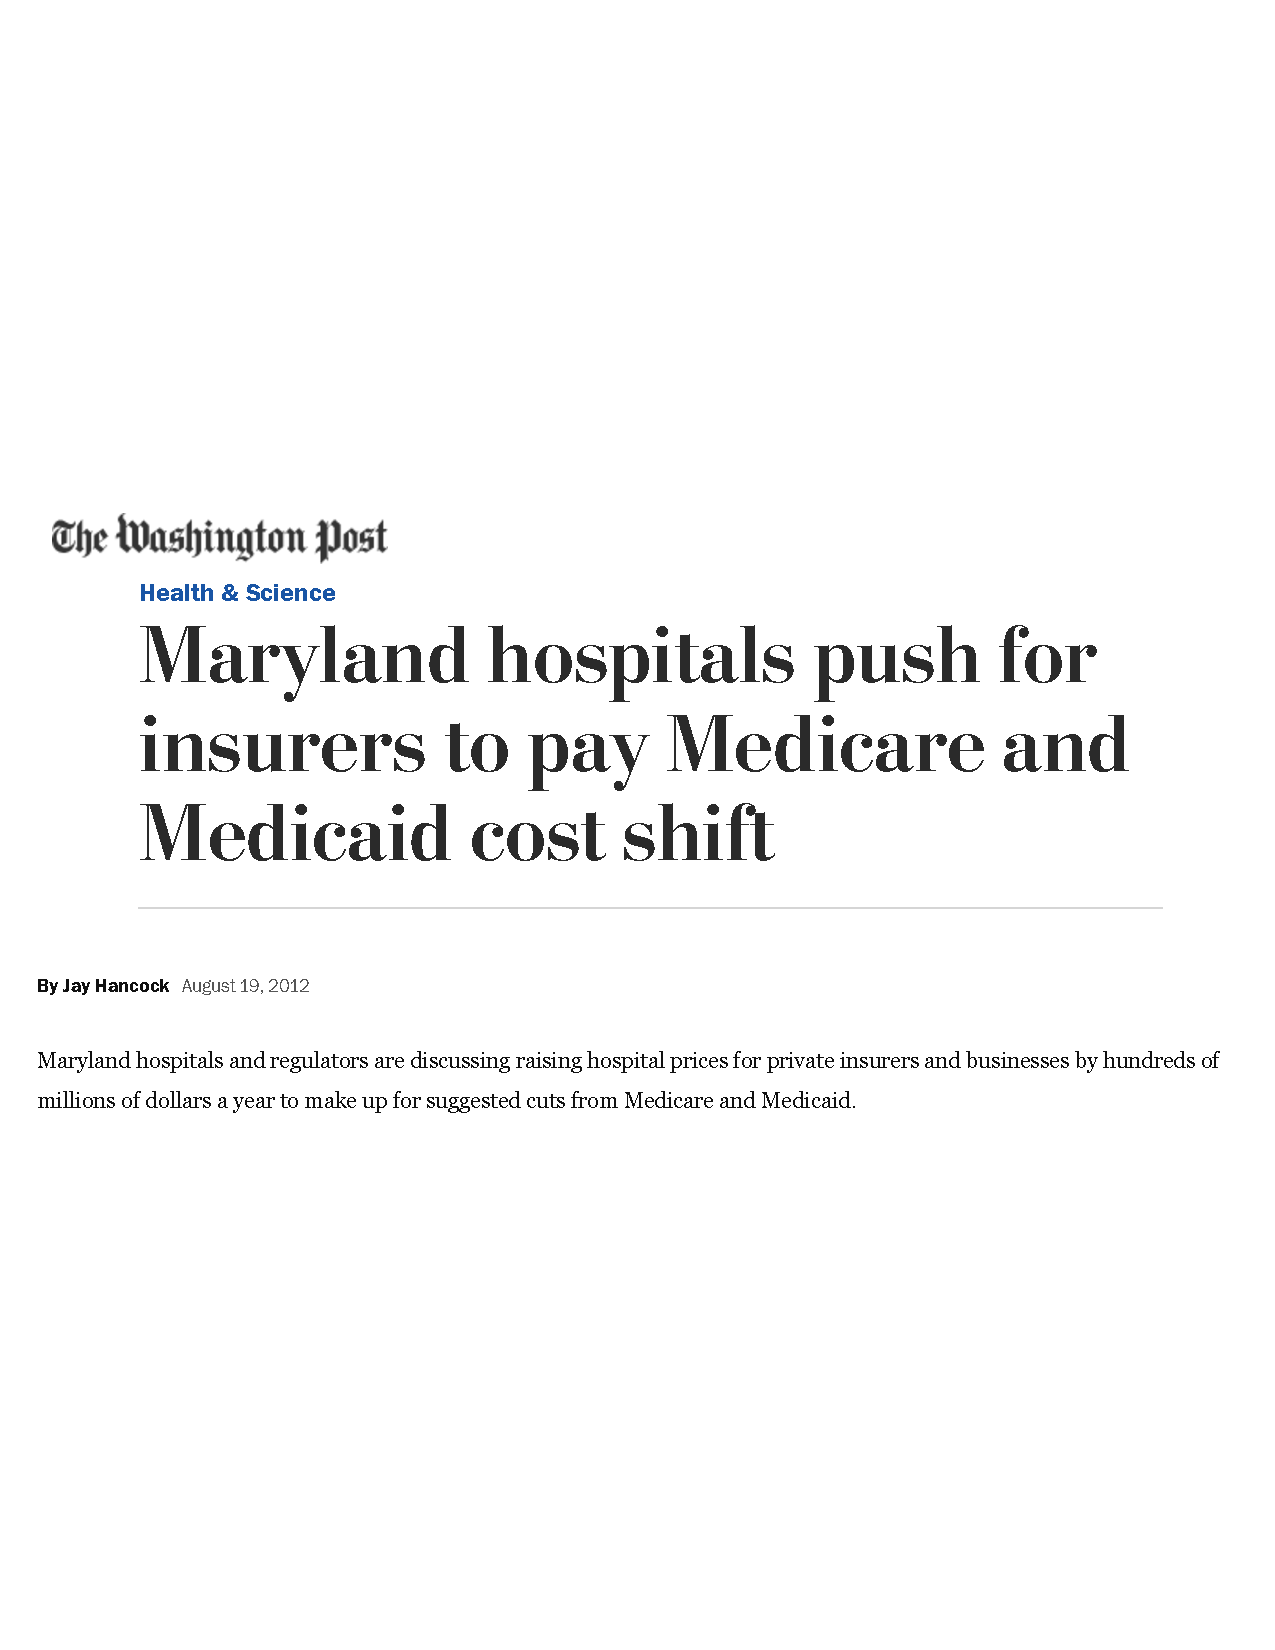
\includegraphics[scale=0.58]{maryland1}
\end{center}
\end{frame}

\begin{frame}
\frametitle{Cont.}
\begin{itemize}
\item ``Cost shifts have been a fact of hospital financial survival for decades.... The data show ...  how private payment is a mirror image of public payment over time and that the cost shift occurs. Hospitals must make up for shortfalls through a combination of approaches and cost-shifting is among them.''
-  -\textcolor{red}{Rich Umbdenstock, Former President and CEO of American Hospital Association}

\end{itemize}
\end{frame}

















\begin{frame}
\frametitle{Medicare Enrollees}
\begin{center}
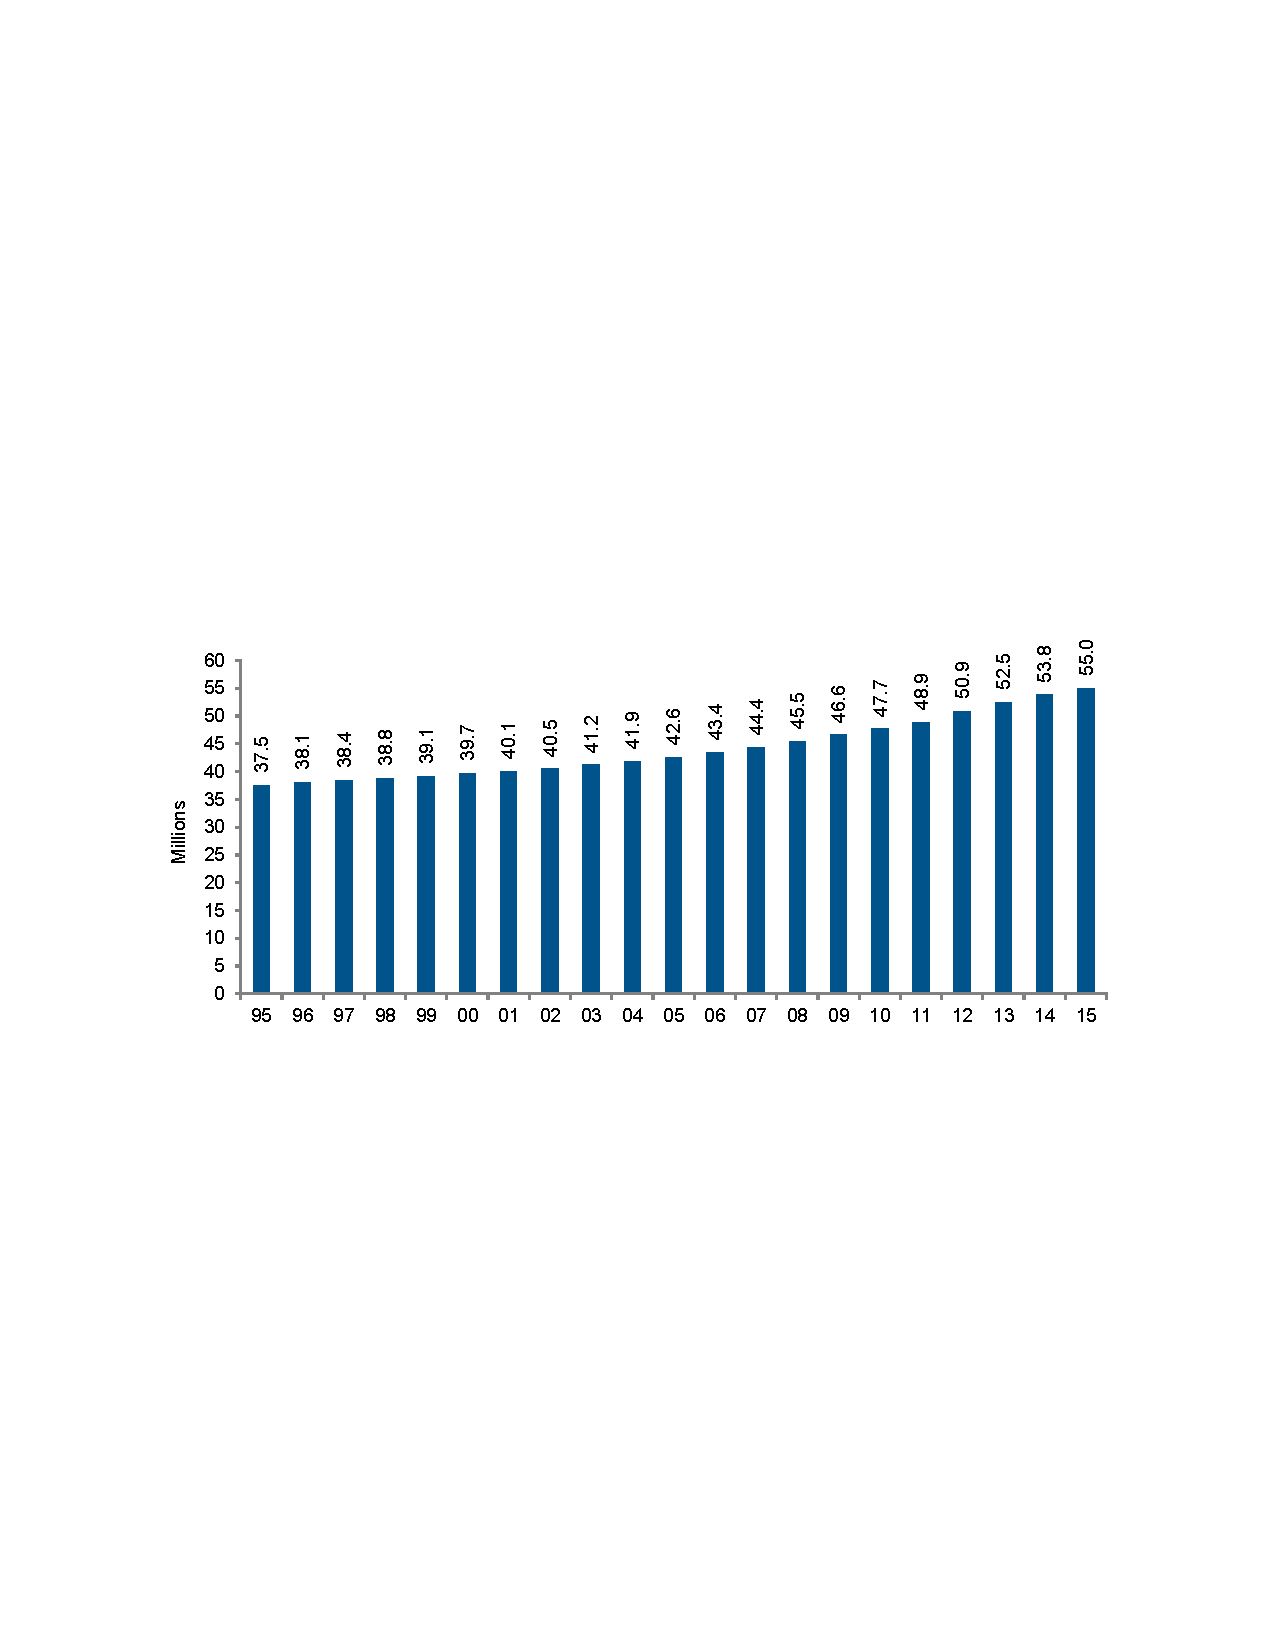
\includegraphics[scale=0.7]{1_17}
\end{center}
\tiny Source: AHA Trendwatch Chartbook 2016.  Data from CMS.
\end{frame}

\begin{frame}
\frametitle{Hospital Cost by Payer Type}
\begin{center}
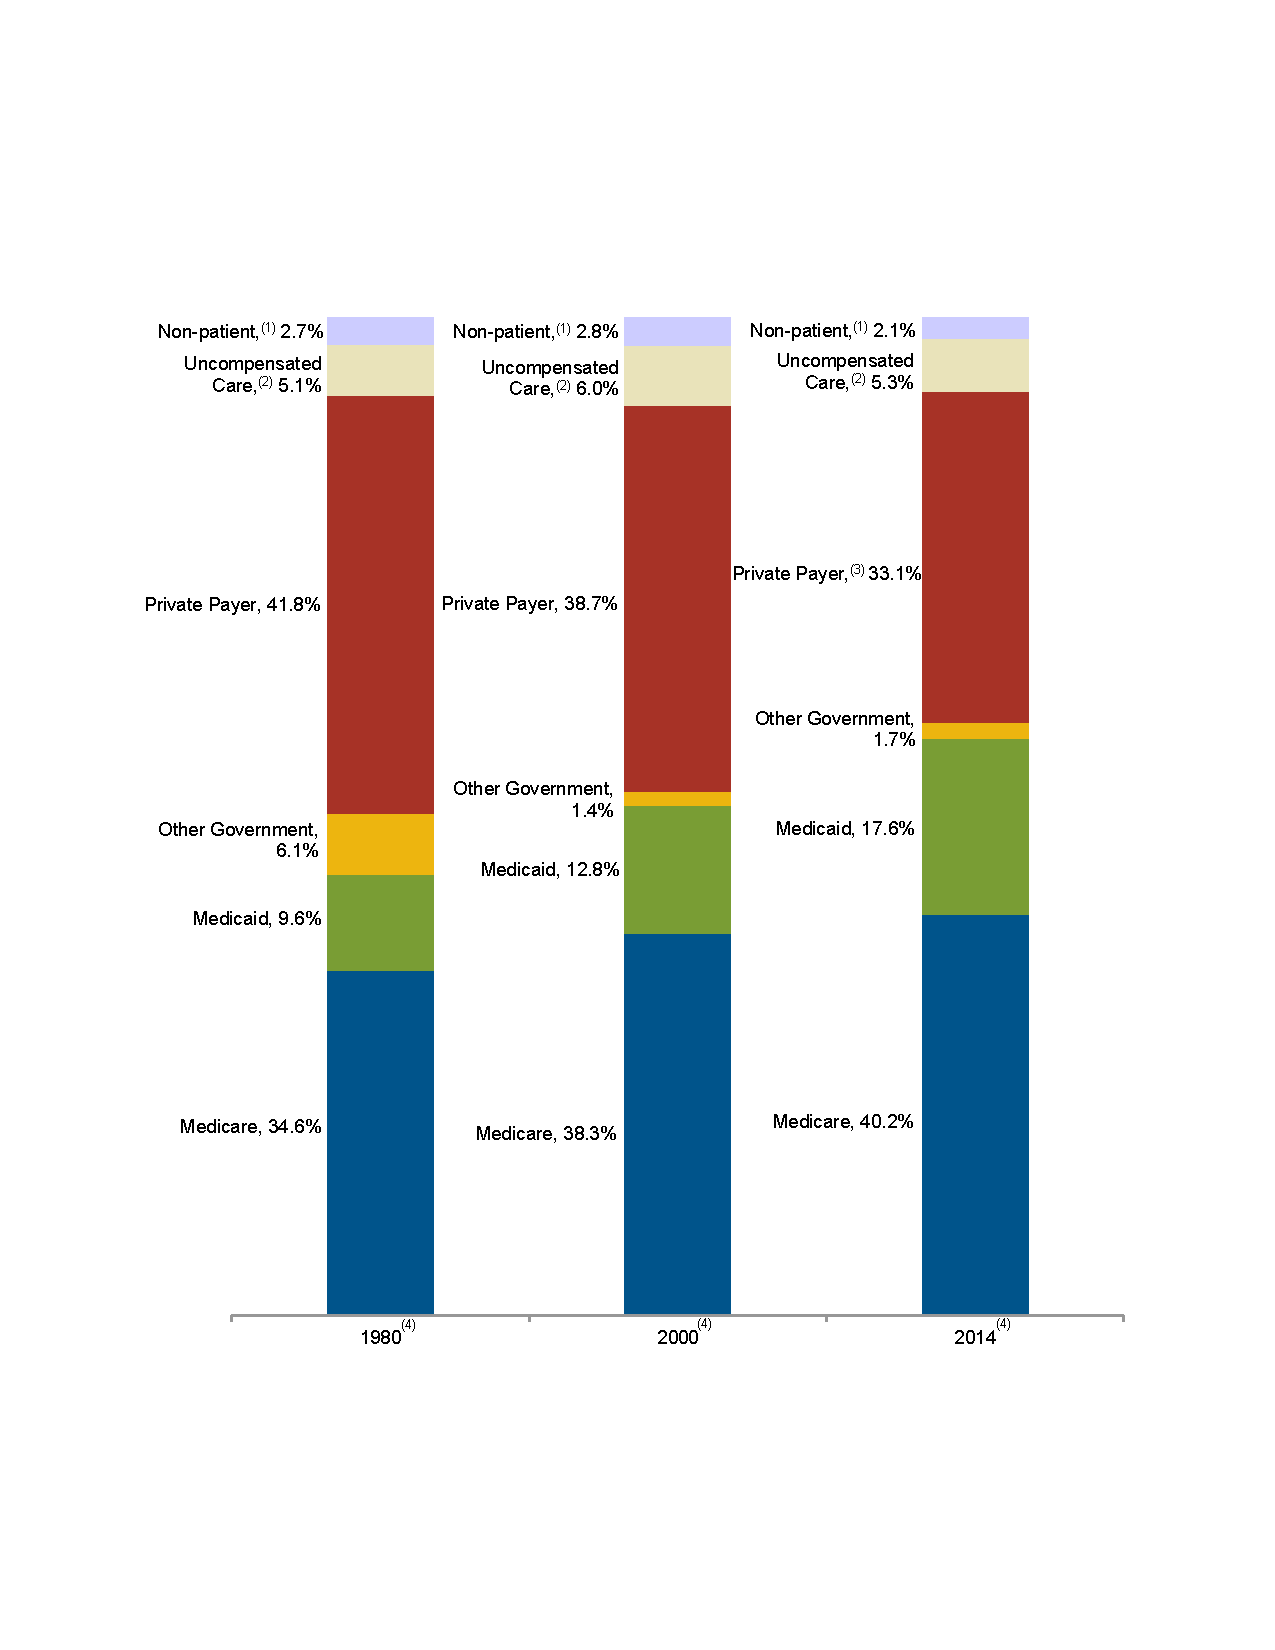
\includegraphics[scale=0.35]{4_5}
\end{center}
\tiny Source: AHA Trendwatch Chartbook 2016.  
\end{frame}
\begin{frame}
\frametitle{Payment Shortfall Relative to Costs}
\begin{center}
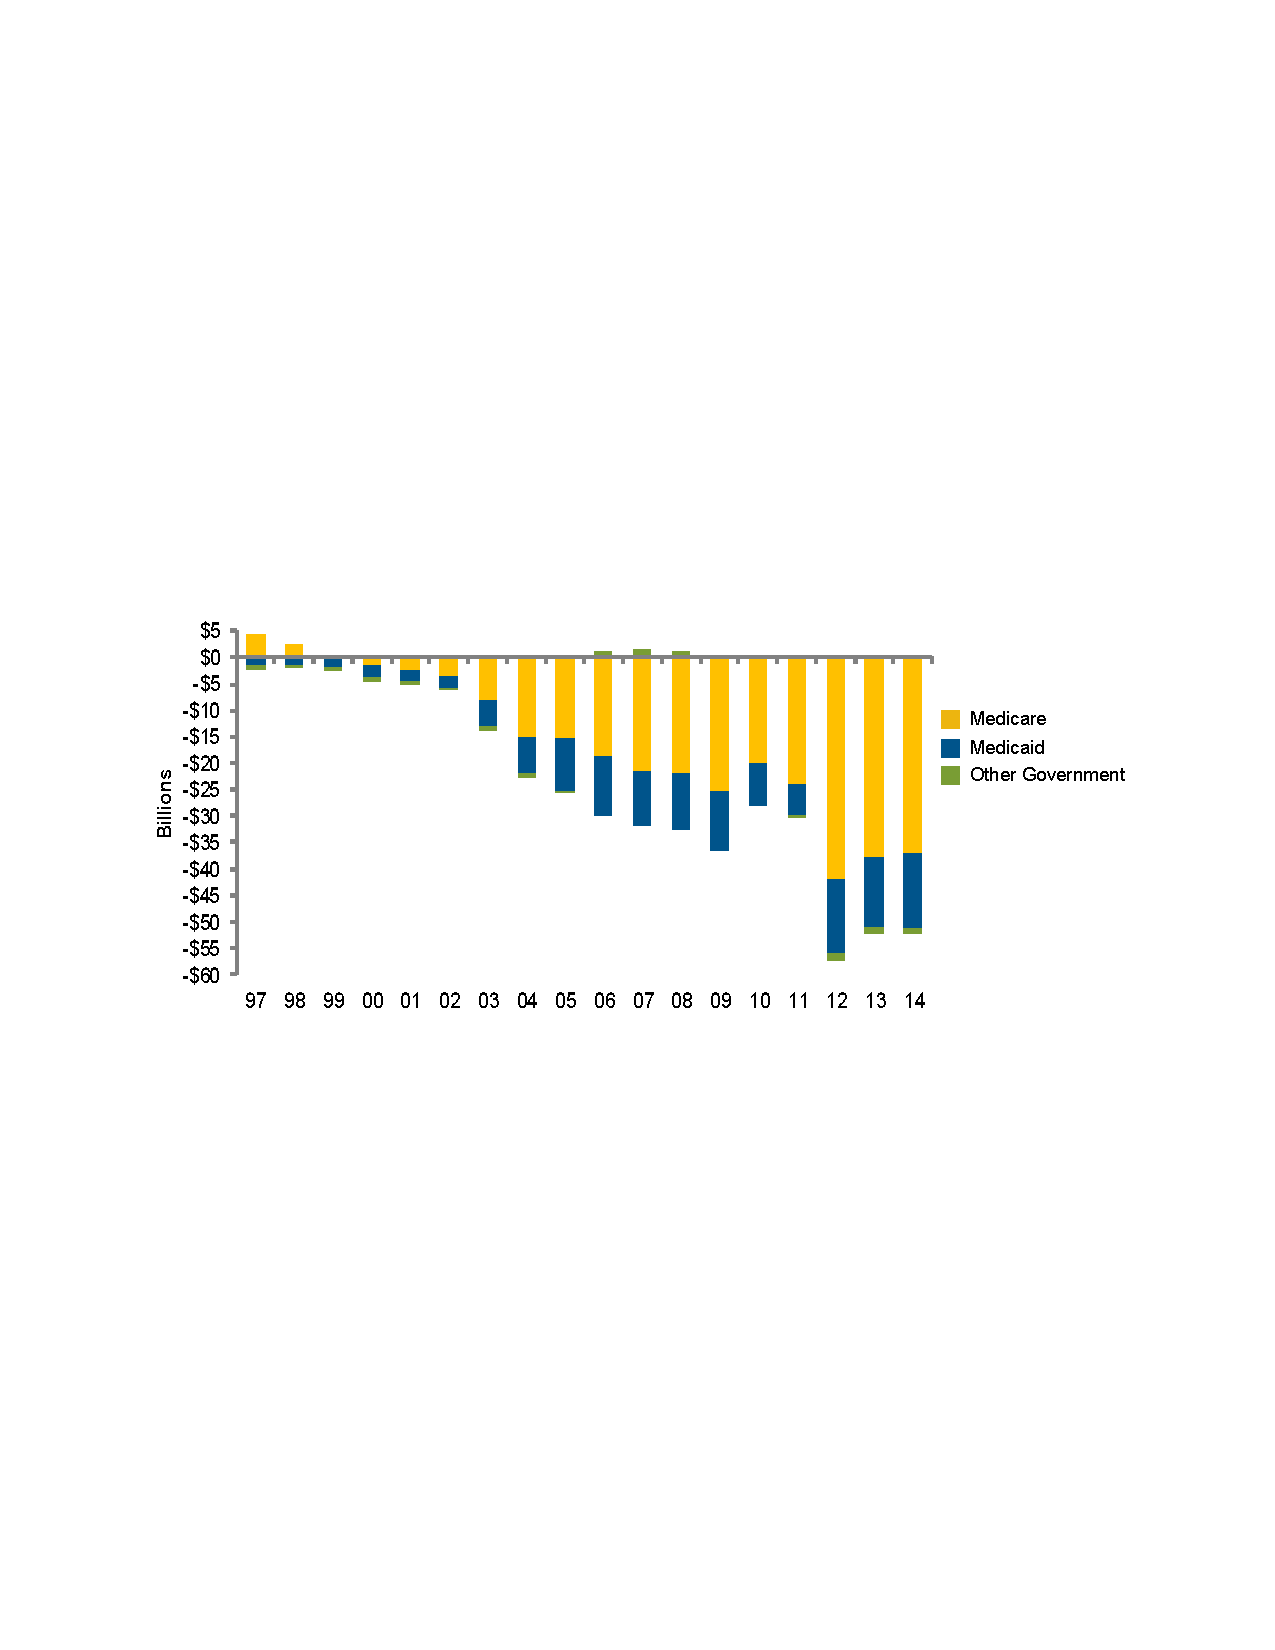
\includegraphics[scale=0.7]{4_7}
\end{center}
\tiny Source: AHA Trendwatch Chartbook 2016.  
\end{frame}

\begin{frame}
\frametitle{Payment-to-Cost Ratios}
\begin{center}
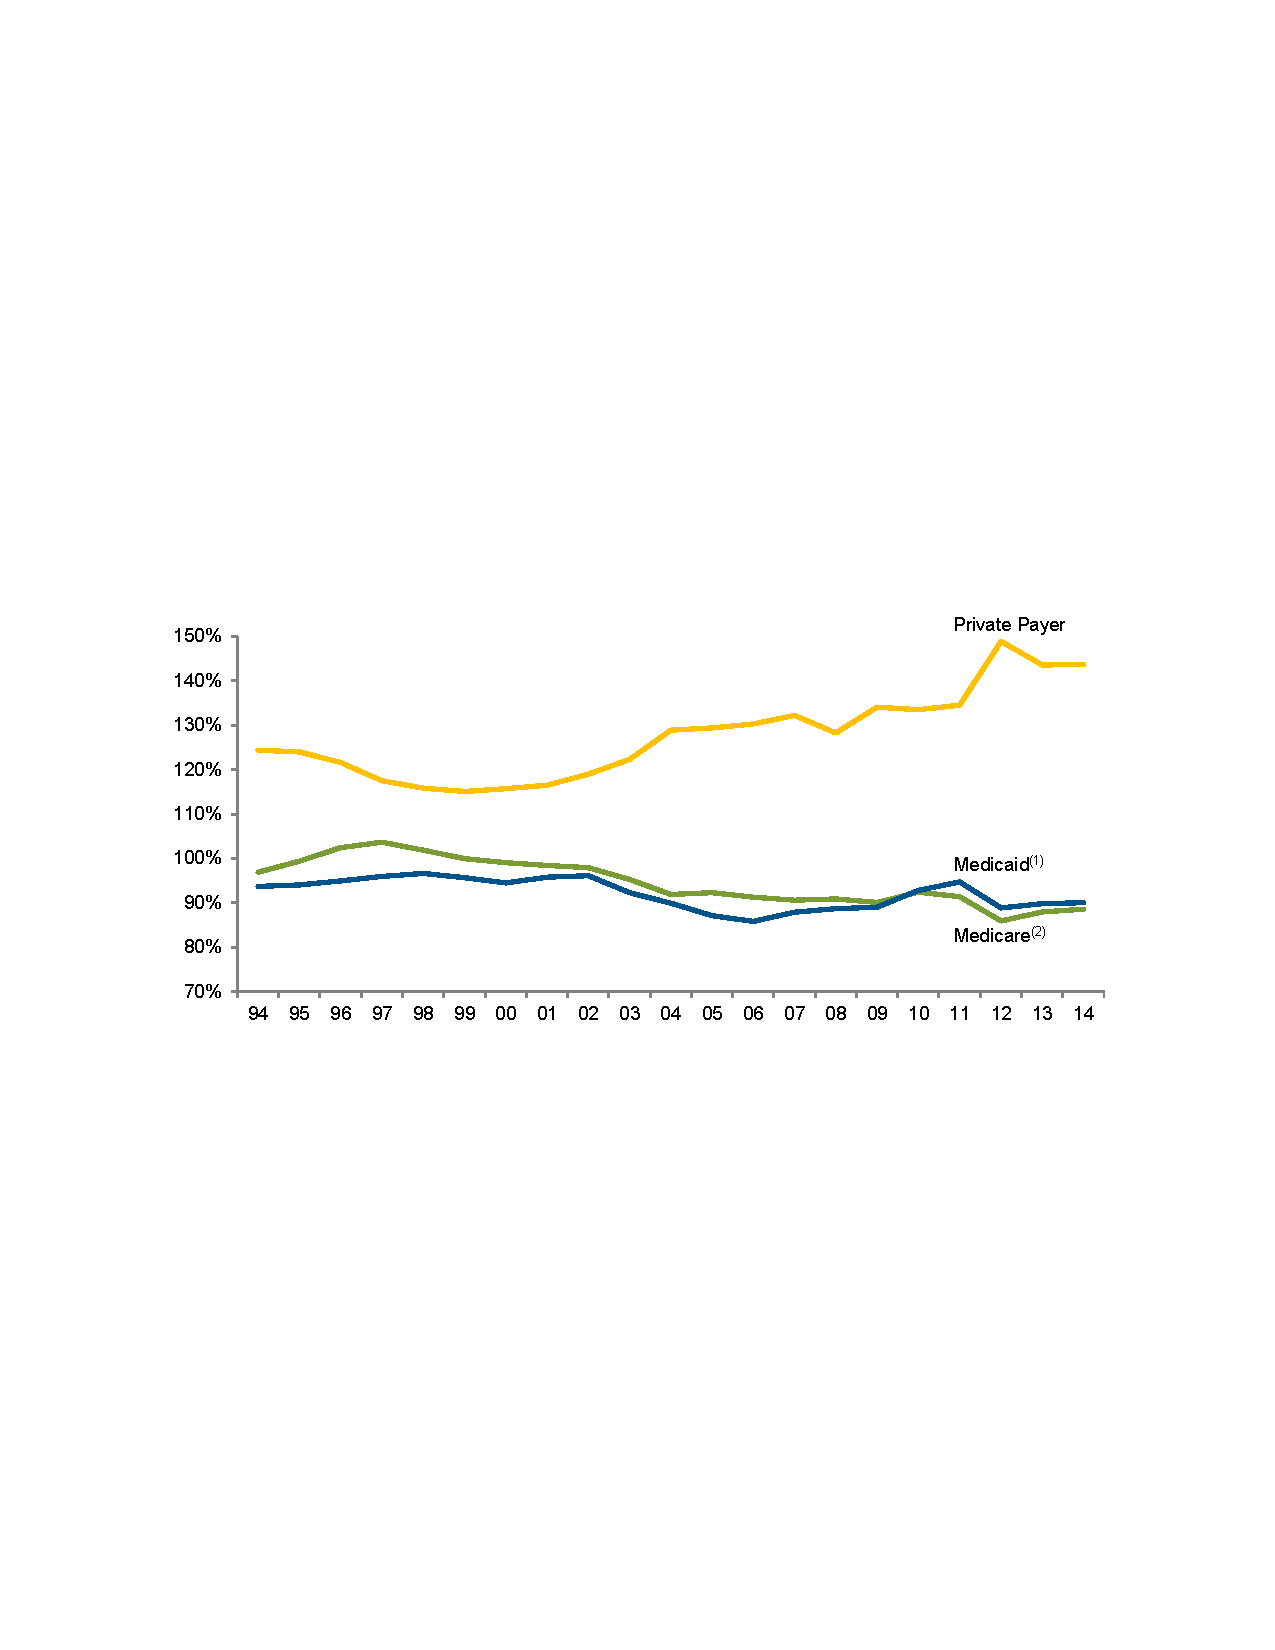
\includegraphics[scale=0.7]{4_6}
\end{center}
\tiny Source: AHA Trendwatch Chartbook 2016.  
\end{frame}


\begin{frame}
\frametitle{Hospital Concentration}
\begin{center}
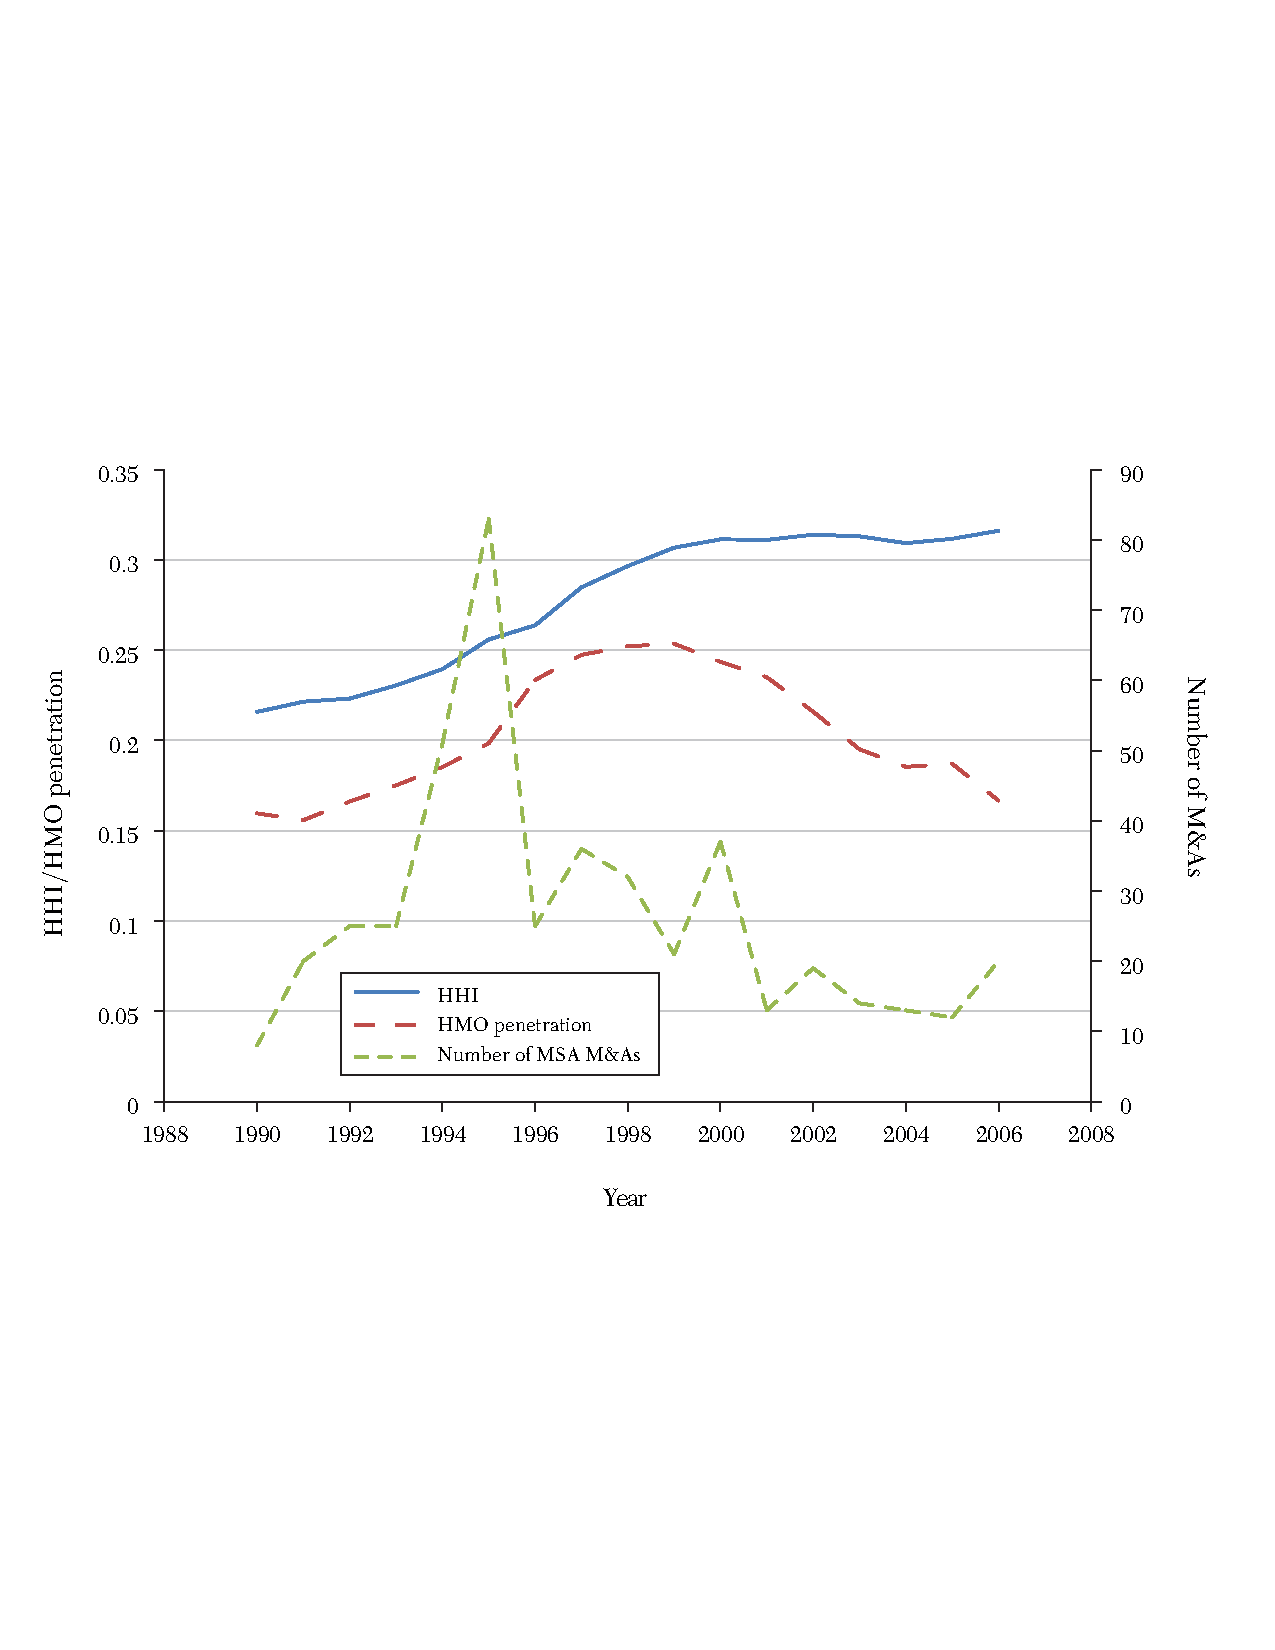
\includegraphics[scale=0.5]{gay1}
\end{center}
\tiny Source: Gaynor, Ho, and Town (2015)
\end{frame}

\begin{frame}
\frametitle{Hospital Concentration}
\begin{center}
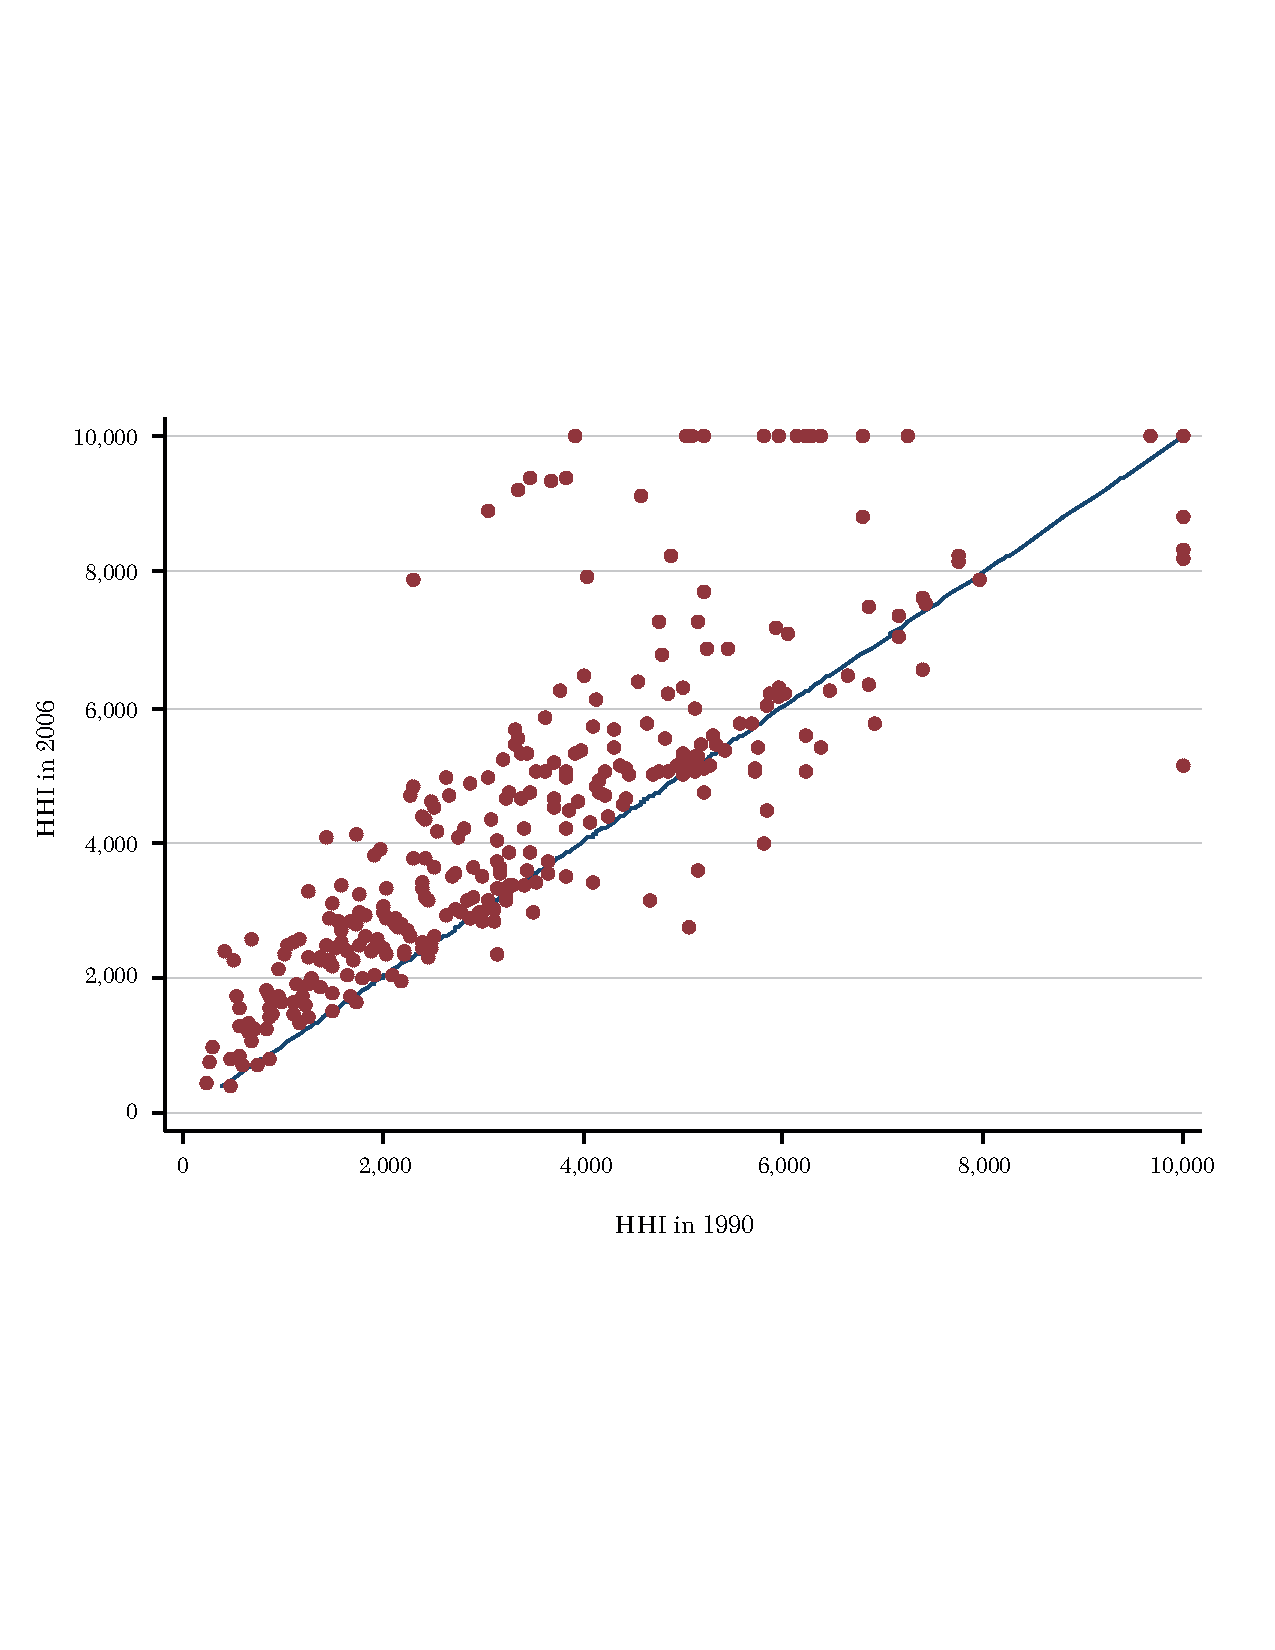
\includegraphics[scale=0.5]{gay2}
\end{center}
\tiny Source: Gaynor, Ho, and Town (2015)
\end{frame}

\begin{frame}
\frametitle{Premiums are Rising}
\begin{center}
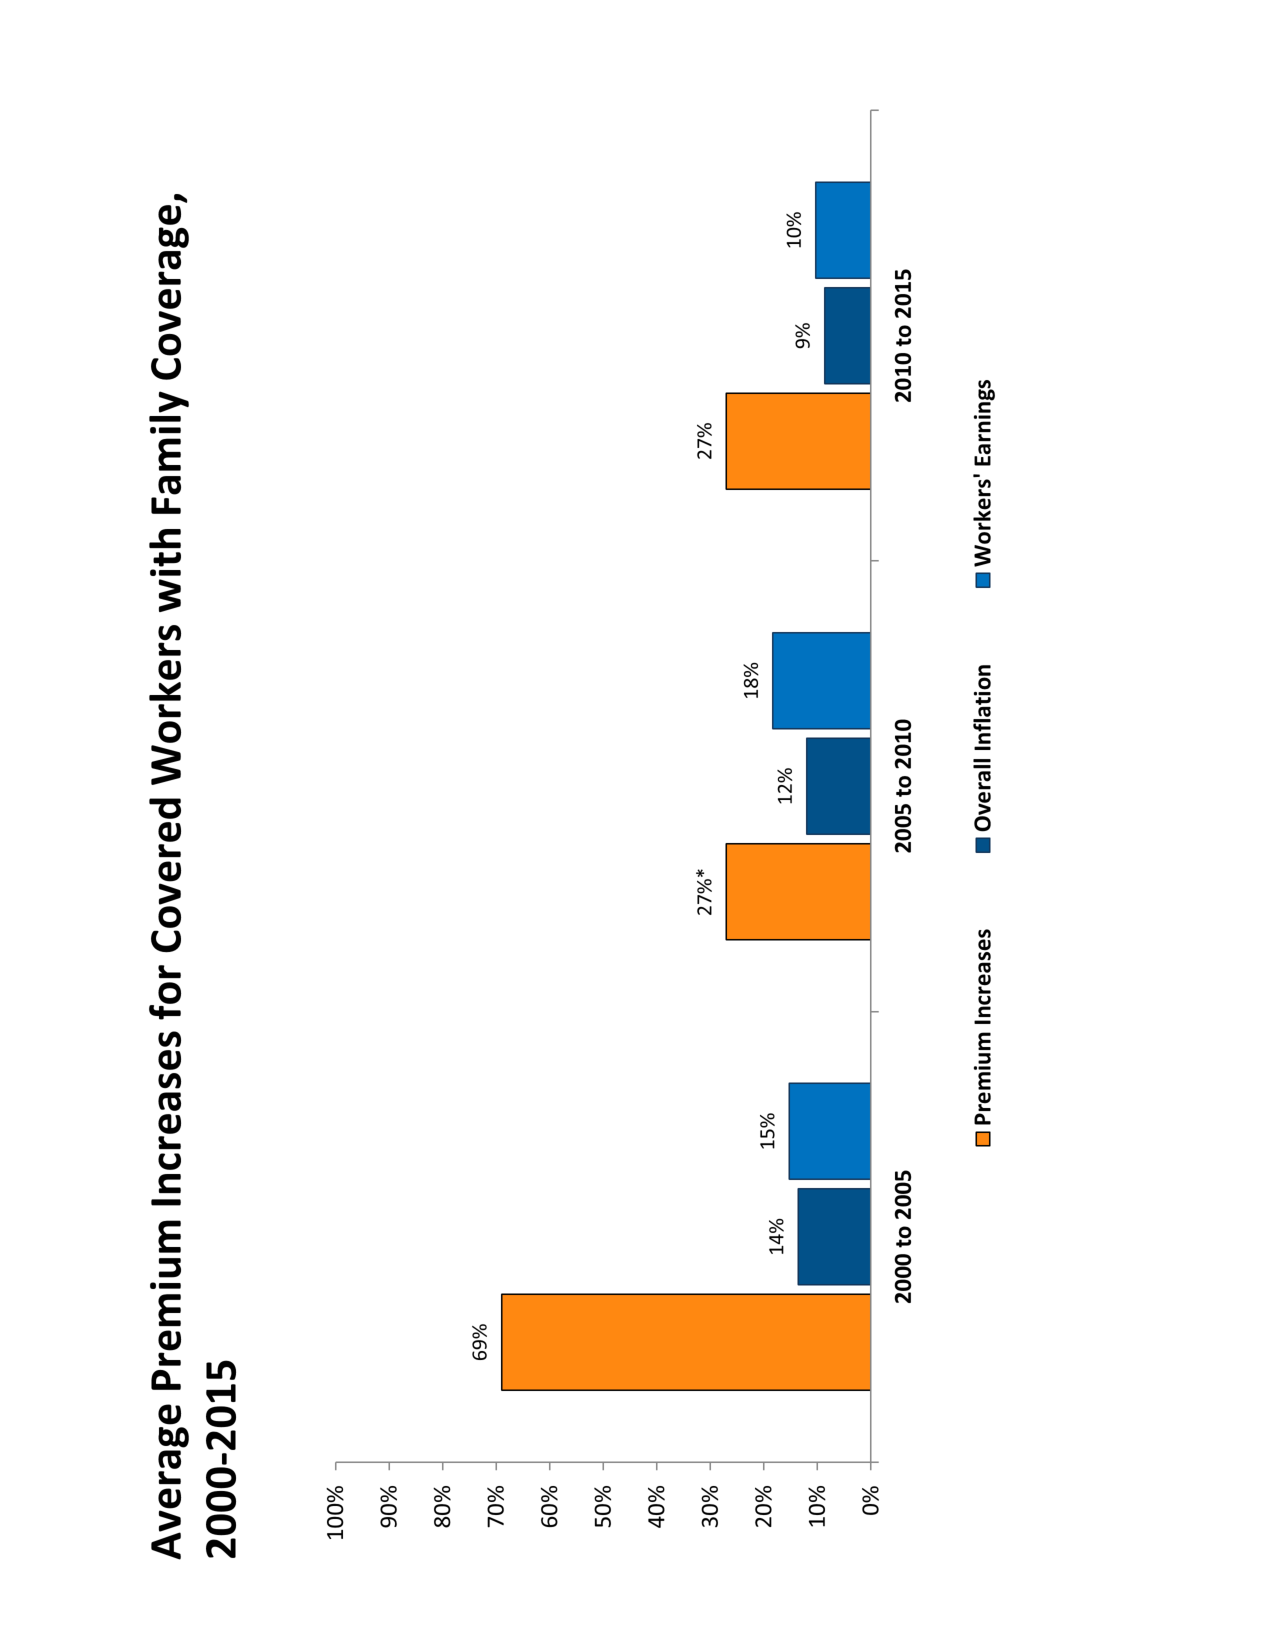
\includegraphics[angle=-90, scale=0.4]{prem}
\end{center}
\tiny Source: Kaiser Family Foundation  
\end{frame}

\begin{frame}
\frametitle{Policy Argument: Uncompensated Care}
"You and I are both paying 900 bucks on average - our families - in higher premiums because of uncompensated care.''  - \textcolor{red}{Barack Obama}
\end{frame}



\begin{frame}
\frametitle{Evidence of Cost-Shifting: ``Sharing the Pain''}
\begin{itemize}
\item Gowrisankaran and Town (1997)
\item Clement (1998)
\item Cutler (1998)
\item  Zwanziger and Bamezai (2000, 2006)
\end{itemize}
\pause
\small Insurance industry funded study by PWC found \textit{massive} cost-shifting! PWC (2010)
\end{frame}



\subsection{Evidence Against Cost-Shifting}





\begin{frame}{Firms Shouldn't Do This!}
``Economists usually presume that a profit-maximizing firm has previously fully exploited
all opportunities to reduce costs or raise revenues, so absent a fundamental rethinking of the firm's
strategy, it would have to absorb the loss.'' -Dranove \textit{et al.} 2017
\end{frame}

\begin{frame}
{\bf Cost-shifiting occurs rarley if at all!}
\begin{itemize}
\item ``In fact, as a whole, the
evidence does not support the notion that cost-shifting is both large and
pervasive. Instead, it reveals that cost-shifting can occur but may not
always do so.When it has occurred, it has generally been measured at a
rate far below dollar-for-dollar'' - \textcolor{red}{Austin Frakt}
\end{itemize}

\end{frame}


\begin{frame}
\frametitle{Simple Economics: Hay 1983}
\pause
\begin{center}
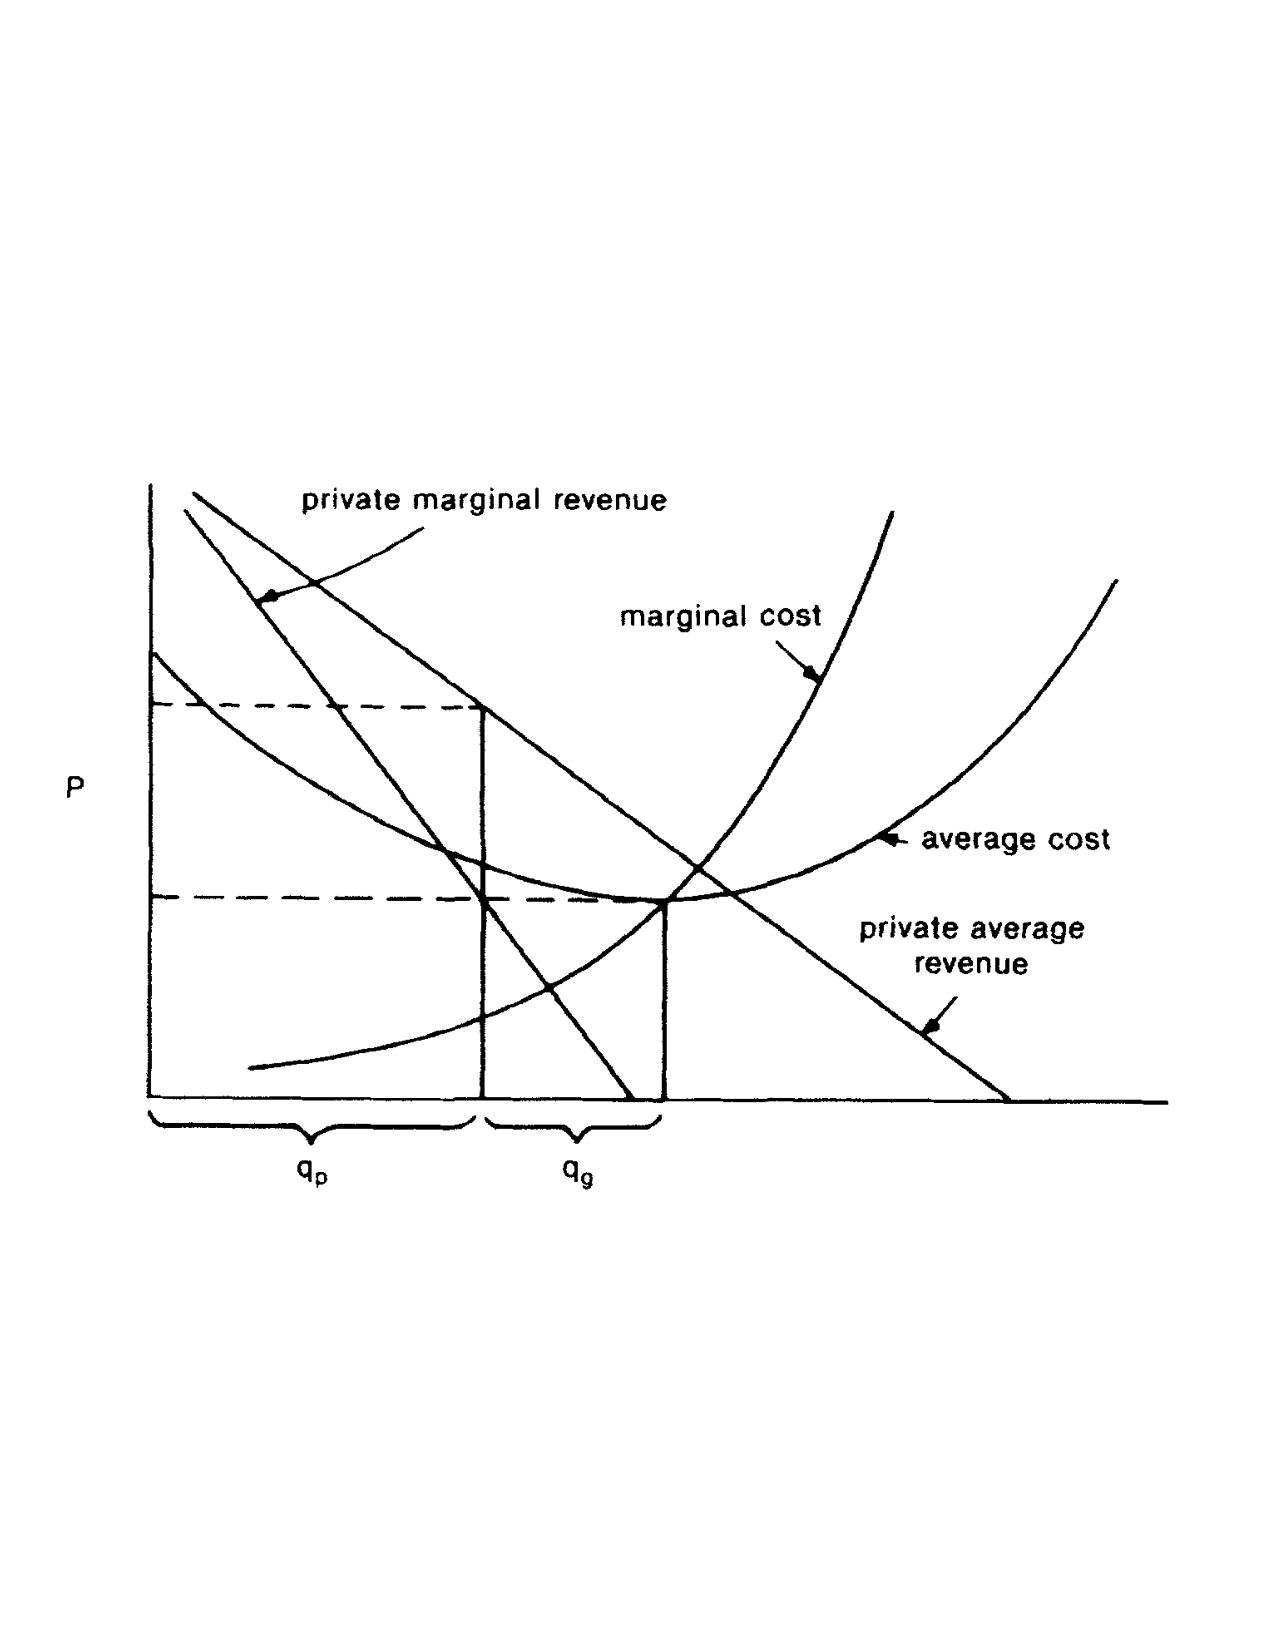
\includegraphics[scale=0.5]{hay}
\end{center}
\tiny Source: Hay (1983)
\end{frame}




%\subsection{Basic Question}








\begin{frame}
\frametitle{Sizable Literature Against Cost-Shifting}
\begin{itemize}
\item Evidence Against Cost-Shifting: 
\begin{itemize}
\item Zero effect: Wu (2010), Dranove (2017)
\item Lower prices: Showalter (1997), Stensland et al. (2010), White (2013)
\end{itemize}
\item Alternative Responses to Public Reimbursement Reductions
\begin{itemize}
\item Lower Profits: Garthwaite (2011)
\item Upcoding:  Dafny (2005)
\item Cutting Costs: Robinson (2011)
\item Heterogeneous Responses: Tai-Seale (1998)
\end{itemize}
\end{itemize}

\end{frame}

\begin{frame}
\frametitle{Why identifying cost-shifiting is difficult?}
Three main reasons:
\begin{enumerate}
\item Complexity of the environment
\item Data Limitations -- 
\begin{itemize}
\item Data on payments from \textit{private insurance} companies to hospitals are typically unobserved.
\item Charge and cost-based measures of prices $\rightarrow$ measurement error!
\end{itemize}   
\item Heterogenous Responses:
\begin{itemize}
\item ``When you've learned how one hospital operates, you've learned how one hospital operates.''
\end{itemize}
\end{enumerate}


\end{frame}








\subsection{Our Contribution}


\begin{frame}{The Questions We Answer}
\begin{enumerate}
\item {\bf Do hospitals respond to public reimbursement cuts by bargaining for higher prices from private insurers?  Do hospitals \textcolor{red}{cost-shift}? }
\pause
\item {\bf What characteristics of hospitals are associated with \textcolor{red}{cost-shifting?}}
\item {\bf Can we rationalize cost-shifting behavior in the modern health care environment for both non-profit and for-profit hospitals?}
\end{enumerate}
\end{frame}




\begin{frame}
\frametitle{Features of Our Analysis}
\begin{itemize}
\item 50$\%$ of all inpatient prospective payment hospitals between 2010 and 2015.
\item Health Care Cost Institute (HCCI) claims data:
\begin{itemize}
\item Aetna, UnitedHealthcare, and Humana.
\item Policies that cover 28$\%$ of Americans under 65 with employer-provided health insurance.
\end{itemize}
\pause
\item Plausibly exogenous variation:
\begin{enumerate}
\item Hospital Readmissions Reduction Program.  (HRRP)
\item Hospital Value Based Purchasing. (HVBP)
%\item[*] Papers like Cutler 1998 use changes in Medicare payment rates over time.  He notes that rates were cut almost every year in the 1980s.  Hospitals may expect cuts.  Furthermore, those cuts were the update factor not keeping up with the market basket whereas we have a discrete cut.
\end{enumerate}

\item Within-hospital price variation.
%\begin{itemize}
%\item Temporal dimension extends cross-sectional work that establishes only price differences (i.e., price discrimination).
%\end{itemize}
\end{itemize}
%% Charges are what the hospital asks for for a patient.  These are rarely what the hospital actually gets because insurance companies pay different amounts for different patients.  Payments, on the other hand, are what hospitals actually receive.  
\end{frame}



%\begin{frame}
%\frametitle{Where we think our paper contributes}
%\begin{itemize}
%\item We use an improved price measure.
%\begin{itemize}
%\item While some papers have transaction prices from a single insurer, we have 60$\%$ of all private insurance transaction prices.  
%\end{itemize}
%\item We exploit a much broader source of cross-sectional variation in reimbursement reductions.
%\item We provide updated results - no studies of the modern health care environment.
%\begin{itemize}
%\item Another reason to revisit this issue is the waive of hospital mergers since the balanced budget act of 1997 (the last major exogenous shock).
%\end{itemize}
%\item Our fixed effects and triple differences methods.
%\end{itemize}
%\end{frame}

\begin{frame}
\frametitle{Findings}
\begin{itemize}
\item Increase in average payments of 1.5$\%$ for hospitals facing a net reimbursement reduction .  Equivalent to:
\begin{itemize}
\item $\$$165 increase in the mean payment between 2013 through 2015.
\end{itemize}
\pause
\item Mean payment effects driven by circulatory and nervous system claims.
\pause
\item Statistically significant results only for non-profit hospitals, but similar magnitude for for-profits.
\pause
\item Significant heterogeneity by payer mix.
\begin{itemize}
\item Hospitals with larger shares of private patients cost-shift more
\end{itemize}
\pause
\item 2.5$\%$ reduction in Medicare Discharges
\end{itemize}
\end{frame}

\begin{frame}{Challenges for our Analysis:}
\begin{itemize}
\item If firms are able to raise prices, why haven't they already?
%\begin{itemize}
%\item Relate our results to theoretical models of market power with different buyer types.  Where \textcolor{red}{could} we see cost-shifting?
%\item Different Objective Functions. Newhouse (1970), Hay (1983), Dranove (1988), McQuire and Pauly (1991), Gowrisankaran and Town (1997)
%\item Expectations about policy reforms.
%\end{itemize}
\item How can firms with "lower quality" be expected to raise price?
%\begin{itemize}
%\item How does the \textcolor{red}{bargaining process} change the posibility for cost-shifting? Dor \textit{et al.} (2004), Gowrisankaran \textit{et al.} (2013)
%\end{itemize}
\item Selection into HRRP and VBP penalties.
%\begin{itemize}
%\item Are trends in prices by penalty status sufficient for identification?
%\item Appropriate triple differences?
%\item Alternative strategies?  "Medicare bite" IV.
%\end{itemize}
\item Financial Crisis of 2008 and Full ACA implementation in 2014.
\end{itemize}
\end{frame}




\section{Empirical Work}
\subsection{Policy Environment}

%\begin{frame}
%\frametitle{What does cutting Medicare really mean?}
%\begin{displaymath}
%\mbox{Medicare Payment}_{ih} = P_{h}*\mbox{DRG Weight}_{h}
%\end{displaymath}
%\end{frame}

%%% Maybe  add a graph for net penalty by something (just so you have two)




\begin{frame}
\frametitle{Motivation of HRRP: Pay for performance}
Prospective Payment System creates incentives for hospitals to discharge patients quickly.  
\pause
\begin{itemize}
%\item Concern about inpatient health.
%\item Medicare pays for readmissions except when the patient returns for treatment of the same condition within 24 h of discharge. 
\item 1.8 million hospitalizations occurring within 30 days of discharge from a prior admission.  
\item Total cost $=$ $\$$24bn 
\item  19.6$\%$ and 28.2$\%$ of all Medicare patients were readmitted within 30 and 60 days, respectively. 
\end{itemize}

\end{frame}




\begin{frame}{Hospital Readmissions Reduction Program}
\begin{table}
\centering
\footnotesize
\begin{tabular}{llll}
\hline \hline
Years penalties applied & FY 2013 & FY2014 & FY2015 \\
\hline
Diagnoses at initial hospitalization & Heart Attack & Heart Attack & Heart Attack \\
						     & Heart Failure & Heart Failure & Heart Failure \\
						     & Pneumonia & Pneumonia & Pneumonia \\
						     & 			&			& Hip and Knee \\
						     &			&			& COPD \\
\hline
Maximum rate of penalty		& 1$\%$ & 2$\%$ & 3$\%$ \\
Average Hospital Payment	& -0.27$\%$ & -0.25$\%$ & -0.49$\%$ \\
\hspace{0.1in} adjustment 	&&& \\
\hspace{0.1in} all hospitals	&&& \\
Average hospital penalty		& -0.42$\%$ & -0.38$\%$ & -0.63$\%$ \\
\hspace{0.1in} adjustment 	&&& \\
\hspace{0.1in} penalized hospitals	&&& \\
Percent of hospitals penalized & 64$\%$ & 66$\%$ & 78$\%$ \\
Percent of hospitals at		&8$\%$ & 0.6$\%$ & 1.2$\%$ \\
\hspace{0.1in} at max penalty	&&& \\
CMS estimate of 			& $\$$290m & $\$$227m & $\$$428m \\
\hspace{0.1in} total penalties &&&\\
\hline
\end{tabular}
\end{table}
\small Penalties: Percentage reduction in base payments on all Medicare inpatient admissions
%Emphasize the timing - lagged 3 years of data.
% Because there are no fixed quality standards and everything is relative to national mean/median, many hospitals have no incentive to change.
\end{frame}





\begin{frame}
\frametitle{HRRP - Cont.}
\begin{displaymath}
\mbox{Excess Readmission Ratio} = \frac{\mbox{risk-adjusted readmissions}}{\mbox{risk-adjusted expected readmissions}}
\end{displaymath}
\begin{itemize}
\item Risk adjustment method adjusted for patient characteristics, %comorbidities, and patient frailty.  
\item Aggregate Payments from Medicare Due to Excess Readmissions.   
\begin{displaymath}
= \sum_{i} (\mbox{base DRG payments}_{i} * (ERR_{i}-1))
\end{displaymath}


\end{itemize}

\end{frame}








\begin{frame}
\frametitle{Evidence from HRRP}
Has HRRP reduced 30-day readmissions?  Improved health outcomes?
\begin{itemize}

\item Mellor \textit{et al.} (2016): HRRP associated with declines in AMI readmission, not due to delay, intensity, or patient mix. 

\item Gupta \textit{et al.} (2018, JAMA Cardiology): 5$\%$ point \textit{increase} in heart failure mortality, despite a reduction in readmissions. 

\item Gupta (2017): 5$\%$ reduction in overall readmissions and 3$\%$ reduction in all-cause mortality. Mostly driven by quality improvement.
\end{itemize}
\end{frame}





\begin{frame}
\frametitle{HVBP Motivation}
%%% Principal-Agent Problem
\begin{itemize}
\item Tie 85$\%$ of fee-for-service Medicare payments to quality or value.
\item The HVBP program scores hospitals:
\begin{itemize}
\item Comparison to other hospitals
\item Comparison to their own previous performance
\end{itemize}
\item Budget neutral:
\begin{itemize}
\item The Hospital VBP Program is funded by reducing participating hospitals' base FY 2017 operating Medicare severity diagnosis-related group (MS-DRG) payments by 2$\%$.
\end{itemize}
\end{itemize}
\end{frame}





\begin{frame}
\frametitle{Value Based Purchasing Program}
Measures $\rightarrow$ Points $\rightarrow$ Total Performance Score $\rightarrow$ $\%$ Bonus $\rightarrow$ $\$$
\pause
\begin{itemize}
\item Quality domains:
\begin{itemize}
\item Clinical Process of Care: 
\item Patient Experience of Care
\item Efficiency and Cost Reduction
\item Spending
\end{itemize}

\item Points relative to national mean and median.  Also within hospital improvement.
% Improvement is key - there affects a wider swath of hospitals.
\item 2013 through 2017, hospitals are docked 1, 1.25, 1.5, 1.75, and 2 percent, respectively.  
\end{itemize}
\end{frame}


\begin{frame}{HVBP Timeline}
\begin{table}
\centering
\begin{tabular}{llllll}
\hline \hline
Fiscal year   &	2013  &	2014  &	2015  &	2016	  &2017 \\
CMS withholds   &	1$\%$	  &1.25$\%$  &	1.5$\%$	  &1.75$\%$  &	2$\%$ \\
Average hospital bonus &	0.23$\%$	&	0.24$\%$	&	0.44$\%$	&	0.66$\%$	&	0.71$\%$ \\
Average hospital penalty &	0.21$\%$&		0.26$\%$	&	0.30$\%$&		0.48$\%$	&	0.48$\%$\\
Top hospital bonus &	0.83$\%$&		0.88$\%$	&	2.09$\%$&		3.02$\%$	&	4.0$\%$\\
Top hospital penalty &		0.90$\%$&		1.14$\%$	&	1.24$\%$&		1.75$\%$	&	1.83$\%$\\
\hline
\end{tabular}
\end{table}
%Above or below standard DRG reimbursement.
\tiny Source: Managed Care analysis of CMS data
\end{frame}




\begin{frame}
\frametitle{HVBP Cont.}
\textcolor{red}{Potential responses:}
\begin{itemize}
\item Vertical and Horizontal Integration.
\item Improve domain specific (overall) quality
\item Different hospitals have vastly different incentives to make improvements in spending or in different quality domains.
\end{itemize}
Norton \textit{et al.} (2016): Hospitals improved quality of care as a result of HVBP, but only for services with the highest marginal incentives to improve quality of care.  
\end{frame}







%\begin{displaymath}
%MFR = \sum^{26}_{m=1} E\Big(\frac{dMeasure_m}{dPatient}\frac{dPoints}{dMeasure}\frac{dTPS}{dPoints}\frac{d\% Bonus}{dTPS}\frac{d \$}{d \%Bonus}\Big)
%\end{displaymath}

%%% Figueroa in BMJ Evidence that HVBP has led to lower mortality rates is lacking. Nations considering similar pay for
%performance programs may want to consider
%alternative models to achieve improved patient
%outcomes









\begin{frame}
\frametitle{Unique Opportunity}
The HRRP/VBP generates \textcolor{red}{unique variation} in public reimbursements in a very complicated market environment.

\end{frame}


%\begin{frame}{Other Cost-Containment Provisions of ACA}
%\begin{itemize}
%\item Disproportionate Share Hospital Payments
%\item Hospital Acquired Conditions
%\item Market Basket Updates
%\item Medicare Durable Medical Equipment
%\item Prescription Drug Rebates
%\end{itemize}
%\end{frame}











\subsection{The Data}










\begin{frame}
\frametitle{Health Care Cost Institute Data}
Unique data opportunity:
\begin{itemize}
\item All claims from 3 national commercial insurers from all 50 states and DC. 
\begin{itemize}
\item Aetna, UnitedHealthcare, and Humana.
\item Policies that cover 28$\%$ of Americans under 65 with employer-provided health insurance.
\item Every claim for acute care admissions
\end{itemize}
\item Prices are risk-adjusted by patient and service mix: 
\begin{itemize}
\item Regress inpatient episode payment divided by DRG weight on gender, age, and dummies for hospital in each year.  
\end{itemize}
%Gowrisankaran, Nevo, and Town (2015) Gaynor and Vogt (2003), and Cooper, et al. (2015)
\end{itemize}
Because medical services are typically bundled, researchers have focused on the average price for the hospital.  
\end{frame}

\begin{frame}
\frametitle{Charges vs. Costs vs. Payments }
\begin{itemize}
\item \textbf{Charges}: The initial, individual list prices a hospital sets for different services. ``Chargemaster.''  
\item \textbf{Costs}: Expenses incurred by a hospital in providing patient care, both direct and indirect.
\item \textbf{Payments}: The amount a hospital actually receives for providing patient care.
\end{itemize}
\begin{table}[htp]
\centering \normalsize
\caption{Per Discharge Correlation Matrix}
\label{tab:corr}

\begin{tabular}{c|ccc}
 		& Cost & Charge & Payment \\
 		\hline
Cost &	1.000		&& \\
Charge &0.382 & 1.000& \\
Payment &0.274&0.435 & 1.000\\
\hline
\end{tabular}
\end{table}
\end{frame}

\begin{frame}
\frametitle{Data Used}
We use data from the following sources:
\begin{itemize}
\item Health Care Cost Institute.
\item Hospital Compare.
\item American Community Survey
\item American Hospital Association (AHA) annual surveys
%\item Hospital level characteristics such as bed count, system membership status, for-profit versus not-for-profit status, and teaching hospital status are from  theAmerican Hospital Association (AHA) annual surveys.
\item Healthcare Cost Report Information System (HCRIS) 
%\item Share of Medicare, Medicaid, and private insurance patients come from the Healthcare Cost Report Information System (HCRIS) database.
\end{itemize}
\end{frame}


\begin{frame}
\frametitle{Environment}
1,386 inpatient prospective payment system hospitals from 2010 to 2015:
\begin{itemize}
\item Smaller hospitals and those without sufficient history (such that HRRP and HVBP don't apply) were dropped.
\item We focus on acute care admissions.
\item Drop all transfer admissions and those in which the patient traveled more than 180 miles.  
\item Claims with incomplete data - likely evidence of procedural errors - are dropped
\item Claims with a payment ratio below the 5th percentile and above the 95th percentile were excluded.
\end{itemize}
\end{frame}

\begin{frame}
\frametitle{Dependent Variables}

\begin{table}[htp]
\centering \normalsize
\caption{Characterization of Research Sample over Time}
\label{tab:samplemort}
\begin{tabular}{cccc}
\hline \hline
%\multicolumn{9}{c}{}\\
Fiscal & Sample 		&  Payment $\$$			& Percent \\
Year   &  Size    		&  Mean (St. Dev.) 			& Penalized \\
 \hline
2010 &      1,386		& 	10,408.18   (9,501.88)	& 0.00  \\
2011 &      1,386		& 	10,517.91   (4,624.22)	& 0.00   \\
2012 & 	1,386 		& 	10,262.14   (4,488.17) 	& 0.32   \\
2013 & 	1,386		& 	10,235.52   (6,682.76)	& 0.74  \\
2014 & 	1,386		&	10,453.04   (4,672.43)	& 0.76 \\
2015 &     1,386		& 	10,984.82   (5,854.48)	& 0.79 \\
&&&\\
\hline
Total & 	8,316		& 10,470.89   (6,272.67)	&	 0.43 \\
\hline
\end{tabular}
\end{table}
\end{frame}


\begin{frame}
\frametitle{Variables by Penalty}

\begin{table}[htp]
\centering \normalsize
\caption{Hospital Characteristics by Penalties}
\label{tab:hosp}
\begin{tabular}{lccc}
\hline \hline
Variable 	& Never 				& Ever  				& p-value  	  \\
		   		&  Penalized    		& Penalized			&       				\\
 \hline
Log(Payment)	&	9.434	&	9.310	&	0.000	\\
System  Membership      	&	0.768	&	0.784	&	0.352	\\
Non-profit     	&	0.790	&	0.692	&	0.000	\\
Log(Case Mix Index)        	&	0.437	&	0.447	&	0.090	\\
\hline
\end{tabular}
\end{table}
\end{frame}





\subsection{Empirical Model}
\begin{frame}
\frametitle{Basic Framework}
Hospital Fixed Effects Estimator: 
\begin{equation}
\label{eq: reg}
y_{hct} = \alpha_{h} + x^{'}_{ht}\beta +  Z^{'}_{ct}\gamma+ \delta1[Penalty]  + \theta_{t}  +  \epsilon_{hct},
\end{equation}
\begin{itemize}
\item $y_{hct} =$ outcome in hospital $y$ in county $c$ in year $t$.
\item $\alpha_{h}=$ hospital fixed effect.
\item $x_{ht}=$ time-varying hospital characteristics.
\item $Z_{ct}=$ time-varying county characteristics.
\item $\theta_{t}=$ year fixed effect.
\item $\epsilon_{hct}=$ i.i.d. across hospitals and time error component.
\end{itemize}
$1[Penalty]$  penalty variable is zero in years 2010 and 2011 for all hospitals.
\end{frame}


\subsection{Basic Findings}

\begin{frame}
\frametitle{Fixed Effects Regression Results}
\begin{table}[htp]
\centering \normalsize
\caption{Baseline Results}
\label{tab:samplemort}
\footnotesize
\begin{tabular}{lllll}
\hline	
 			& Log Mean				& Log Medicaid 	   	& Log Medicare   		& Log Private  			\\
			& Payment				& Discharges      		& Discharges       		& Discharges        	\\
\hline
Net Penalty  	&	0.015***		&	-0.044**	&	-0.025***	&	-0.002	\\
	&	(0.005)		&	(0.021)	&	(0.006)	&	(0.010)	\\
\hline
\tiny Notes: $n=8,316$.  
\end{tabular}
\end{table}
\tiny All regressions include hospital and year fixed effects and other hospital level controls include bed count and labor force.  Market power variables are constructed as the overall county market share tercile.  Large market is a binary variable for a hospital in the top half of the market size distribution.  In cases in which independent variables are missing, we recode them and control for missing variable indicators to ensure a balanced panel.  Standard errors are clustered at the hospital level.  *** p-value$<$0.01, ** p-value$<$0.05, * p-value$<$0.1.
\end{frame}

\begin{frame}
\frametitle{Fixed Effects Regression Results}
\begin{table}[htp]
\centering \normalsize
\caption{Baseline Results}
\label{tab:samplemort}
\footnotesize
\begin{tabular}{llllll}
\hline	
 			& Log Mean		& Log Mean		& Log Medicaid 	   	& Log Medicare   		& Log Private  			\\
			& Payment		& 	Charge		& Discharges      		& Discharges       		& Discharges        	\\
\hline
Net Penalty  	&	0.015***	&	0.008	&	-0.044**	&	-0.025***	&	-0.002	\\
	&	(0.005)	&	(0.008)	&	(0.021)	&	(0.006)	&	(0.010)	\\
\hline
\tiny Notes: $n=8,316$.  
\end{tabular}
\end{table}
\tiny All regressions include hospital and year fixed effects and other hospital level controls include bed count and labor force.  Market power variables are constructed as the overall county market share tercile.  Large market is a binary variable for a hospital in the top half of the market size distribution.  In cases in which independent variables are missing, we recode them and control for missing variable indicators to ensure a balanced panel.  Standard errors are clustered at the hospital level.  *** p-value$<$0.01, ** p-value$<$0.05, * p-value$<$0.1.
\end{frame}


\begin{frame}
\frametitle{Event Study}
\begin{center}
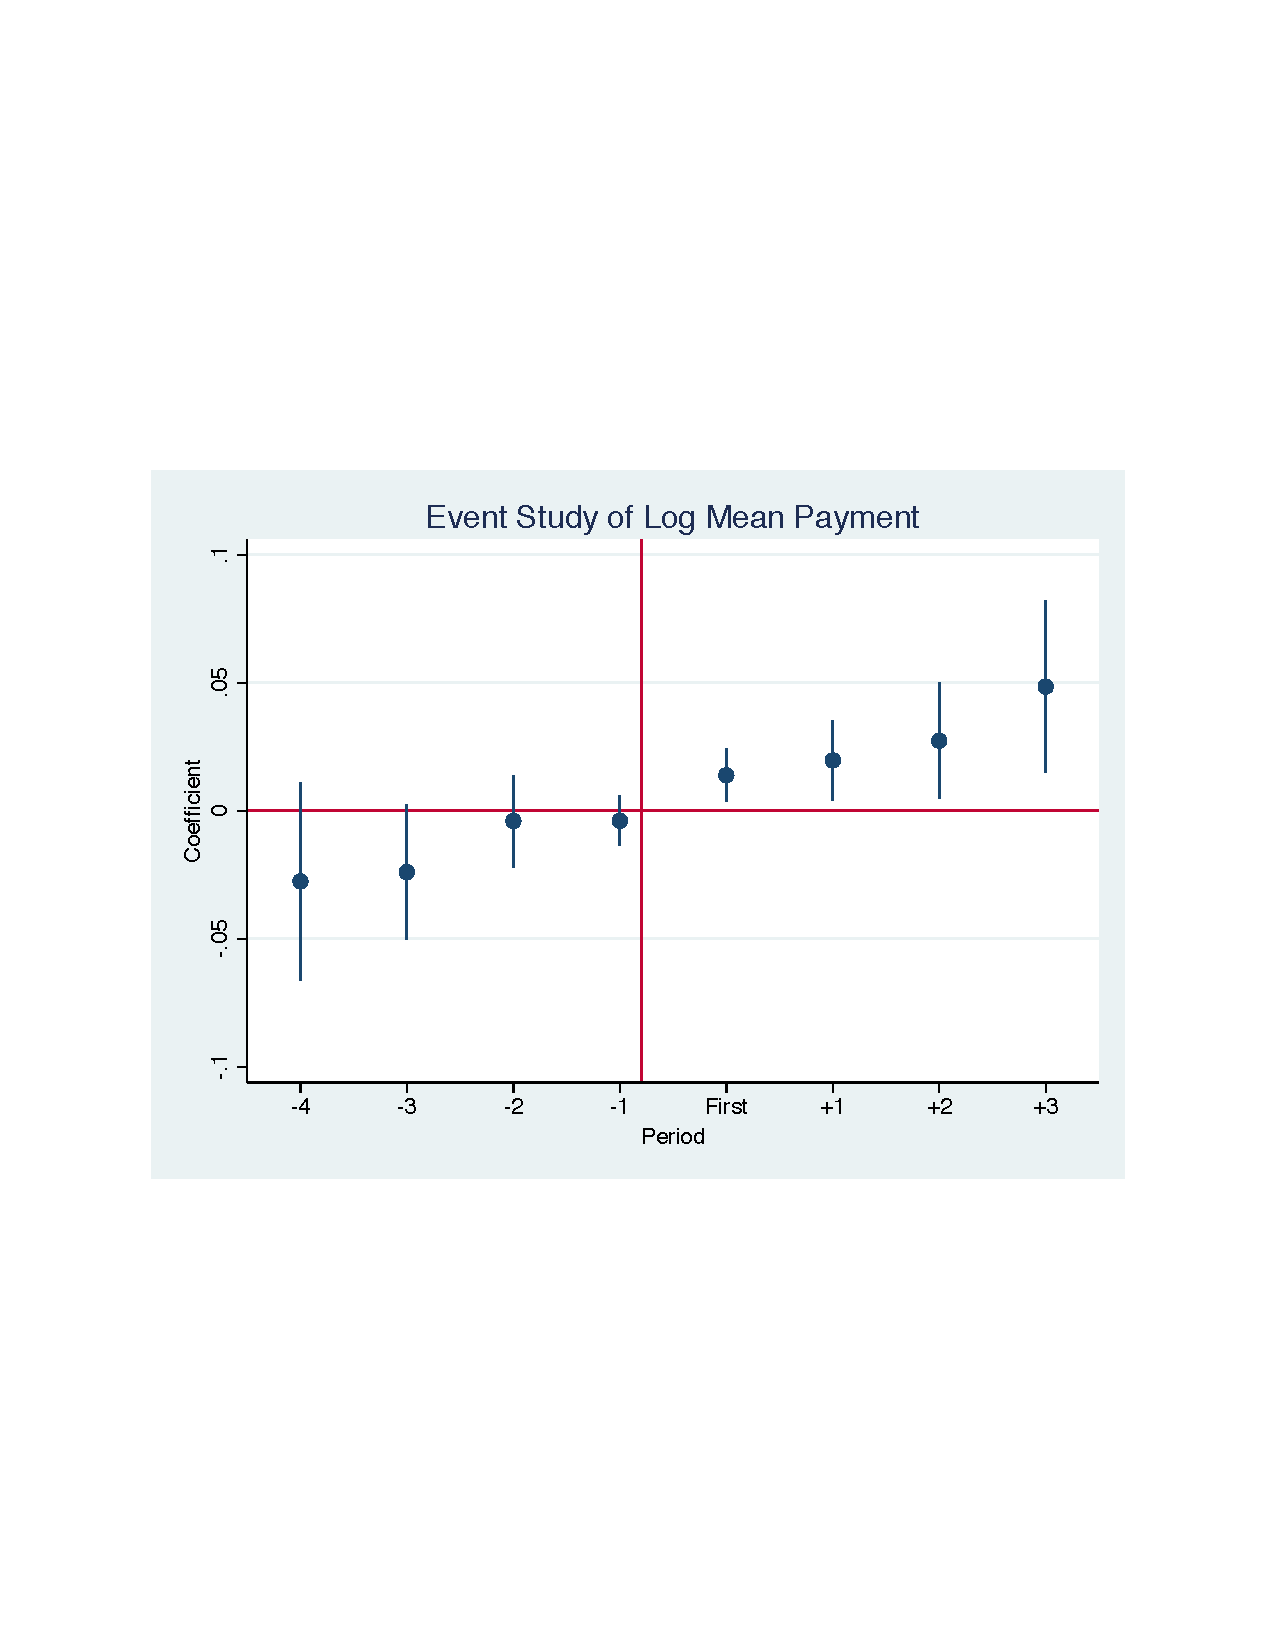
\includegraphics[scale=0.55]{event}
\end{center}
\end{frame}


\begin{frame}
\frametitle{Fixed Effects Regression Results: Intensive Margin}
\begin{table}[htp]
\centering \normalsize
\caption{Baseline Results}
\label{tab:samplemort}
\footnotesize
\begin{tabular}{llllll}
\hline	
 			& Log Mean		& Log Mean		& Log Medicaid 	   	& Log Medicare   		& Log Private  			\\
			& Payment		& 	Charge		& Discharges      		& Discharges       		& Discharges        	\\
\hline
Large Bonus	&	-0.006	&	0.017	&	0.023	&	0.027**	&	0.043***	\\
			&	(0.008)	&	(0.012)	&	(0.034)	&	(0.012)	&	(0.016)	\\
Low Penalty	&	0.011*	&	0.014	&	-0.023	&	-0.014	&	0.008	\\
			&	(0.006)	&	(0.010)	& 	(0.029)	&	(0.01	0)	&	(0.015)	\\
Large Penalty	&	0.013*	&	0.017	&	-0.046	&	-0.008	&	0.036**	\\
			&	(0.007)	&	(0.012)	&	(0.03	0) 	&	(0.010)	&	(0.015)	\\
\hline
\tiny Notes: $n=8,316$.  
\end{tabular}
\end{table}
\tiny All regressions include hospital and year fixed effects and other hospital level controls include bed count and labor force.  Market power variables are constructed as the overall county market share tercile.  Large market is a binary variable for a hospital in the top half of the market size distribution.  In cases in which independent variables are missing, we recode them and control for missing variable indicators to ensure a balanced panel.  Standard errors are clustered at the hospital level.  *** p-value$<$0.01, ** p-value$<$0.05, * p-value$<$0.1.
\end{frame}


\begin{frame}
\frametitle{Fixed Effects Regression Results: Intensive Margin 2}
\begin{table}[htp]
\centering \normalsize
\caption{Baseline Results}
\label{tab:samplemort}
\footnotesize
\begin{tabular}{llllll}
\hline	
 			& Log Mean		& Log Mean		& Log Medicaid 	   	& Log Medicare   		& Log Private  			\\
			& Payment		& 	Charge		& Discharges      		& Discharges       		& Discharges        	\\
\hline
Penalty ($\$$10k) &	0.000	&	0.000	&	0.000	&	0.000	&	0.000	\\
	&	(0.000)	&	(0.000)	&	(0.000)	&	(0.000)	&	(0.000)	\\
Penalty ($\$$1m) 	&	0.008	&	0.016	&	-0.050	&	0.003	&	0.023	\\
	&	(0.009)	&	(0.020)	&	(0.031)	&	(0.011)	&	-(0.015)	\\
Penalty ($\$$10m)	&	0.076	&	0.158	&	-0.500	&	0.029	&	0.226	\\
	&	(0.095)	&	(0.202)	&	(0.307)	&	(0.111)	&	(0.146)	\\
\hline
\tiny Notes: $n=8,316$.  
\end{tabular}
\end{table}
\tiny All regressions include hospital and year fixed effects and other hospital level controls include bed count and labor force.  Market power variables are constructed as the overall county market share tercile.  Large market is a binary variable for a hospital in the top half of the market size distribution.  In cases in which independent variables are missing, we recode them and control for missing variable indicators to ensure a balanced panel.  Standard errors are clustered at the hospital level.  *** p-value$<$0.01, ** p-value$<$0.05, * p-value$<$0.1.
\end{frame}







\begin{frame}
\frametitle{Robustness Check 1}
\begin{table}[htp]
\centering \normalsize
\caption{Penalty Specific Trends Results}
\footnotesize
\begin{tabular}{llllll}
\hline	
\hline
 			& Log Mean 		& Log Mean	& Medicaid 	   	& Medicare   		& Private  			\\
			& Payment		& 	Charge	& Discharges      	& Discharges       	& Discharges    \\
											\\
\hline											
Net Penalty 	&	0.010**	&	0.018**	&	-0.037	&	-0.024***	&	-0.008	\\
	&	(0.005)	&	(0.008)	&	(0.023)	&	(0.006)	&	(0.011)	\\
p-value & 0.473 & 0.034 & 0.282 & 0.003 & 0.182 \\
\hline
\end{tabular}
\end{table}
\tiny Notes: Further controls include those in our baseline specification for mean payments.  The p-value in the first row of results is in reference to the null hypothesis that trends in the outcome of interest are the same between ever-penalized and never-penalized hospitals conditional on the model covariates.  In cases in which independent variables are missing, we recode them and control for missing variable indicators to ensure a balanced panel.  Standard errors are clustered at the hospital level.  *** p-value$<$0.01, ** p-value$<$0.05, * p-value$<$0.1.
\end{frame}


\begin{frame}
\frametitle{Robustness Check 2}
\begin{table}[htp]
\centering \normalsize
\caption{Hospital, Year, and County Fixed Effects}
\footnotesize
\begin{tabular}{llllll}
\hline	
\hline
 			& Log Mean 		& Log Mean	& Medicaid 	   	& Medicare   		& Private  			\\
			& Payment		& 	Charge	& Discharges      	& Discharges       	& Discharges    \\
\hline											
Net Penalty 	&	0.016***	&	0.008	&	-0.047**	&	-0.024***	&	0.000	\\
	&	(0.005)	&	(0.008)	&	(0.022)	&	(0.007)	&	(0.010)	\\
	\hline
\end{tabular}
\end{table}
\tiny Notes: Further controls include those in our baseline specification for mean payments.  The p-value in the first row of results is in reference to the null hypothesis that trends in the outcome of interest are the same between ever-penalized and never-penalized hospitals conditional on the model covariates.  In cases in which independent variables are missing, we recode them and control for missing variable indicators to ensure a balanced panel.  Standard errors are clustered at the hospital level.  *** p-value$<$0.01, ** p-value$<$0.05, * p-value$<$0.1.
\end{frame}



\begin{frame}
\frametitle{Robustness Check 3}
\begin{table}[htp]
\centering \normalsize
\caption{Controlling for Medicaid Expansion States}
\footnotesize
\begin{tabular}{llllll}
\hline	
\hline
 			& Log Mean 		& Log Mean	& Medicaid 	   	& Medicare   		& Private  			\\
			& Payment		& 	Charge	& Discharges      	& Discharges       	& Discharges    \\
\hline											
Net Penalty 	&	0.015***	&	0.008	&	-0.042**	&	-0.025***	&	-0.002	\\
	&	(0.005)	&	(0.008)	&	(0.021)	&	(0.006)	&	(0.010)	\\
	\hline
\end{tabular}
\end{table}
\tiny Notes: Further controls include those in our baseline specification for mean payments.  The p-value in the first row of results is in reference to the null hypothesis that trends in the outcome of interest are the same between ever-penalized and never-penalized hospitals conditional on the model covariates.  In cases in which independent variables are missing, we recode them and control for missing variable indicators to ensure a balanced panel.  Standard errors are clustered at the hospital level.  *** p-value$<$0.01, ** p-value$<$0.05, * p-value$<$0.1.
\end{frame}



\begin{frame}
\frametitle{Robustness Check 4}
\begin{table}[htp]
\centering \normalsize
\caption{Controlling for Overall HCAHPS Hospital Rating}
\footnotesize
\begin{tabular}{llllll}
\hline	
\hline
 			& Log Mean 		& Log Mean	& Medicaid 	   	& Medicare   		& Private  			\\
			& Payment		& 	Charge	& Discharges      	& Discharges       	& Discharges    \\
									
\hline											
Net Penalty 	&	0.015***	&	0.007	&	-0.044**	&	-0.024***	&	-0.001	\\
	&	(0.005)	&	(0.008)	&	(0.021)	&	(0.006)	&	(0.010)	\\
\end{tabular}
\end{table}
\tiny Notes: Further controls include those in our baseline specification for mean payments.  The p-value in the first row of results is in reference to the null hypothesis that trends in the outcome of interest are the same between ever-penalized and never-penalized hospitals conditional on the model covariates.  In cases in which independent variables are missing, we recode them and control for missing variable indicators to ensure a balanced panel.  Standard errors are clustered at the hospital level.  *** p-value$<$0.01, ** p-value$<$0.05, * p-value$<$0.1.
\end{frame}



\begin{frame}
\frametitle{Robustness Check 5}
\begin{table}[htp]
\centering \normalsize
\caption{Dropping Fiscal 2012}
\footnotesize
\begin{tabular}{llllll}
\hline	
\hline
 			& Log Mean 		& Log Mean	& Medicaid 	   	& Medicare   		& Private  			\\
			& Payment		& 	Charge	& Discharges      	& Discharges       	& Discharges    \\
\hline											
Net Penalty 	&	0.013**	&	0.009	&	-0.045*	&	-0.024***	&	-0.003	\\
		&(0.005)	&	(0.009)		&(0.023)		&(0.007)	&	(0.011)	\\
\end{tabular}
\end{table}
\tiny Notes: Further controls include those in our baseline specification for mean payments.  The p-value in the first row of results is in reference to the null hypothesis that trends in the outcome of interest are the same between ever-penalized and never-penalized hospitals conditional on the model covariates.  In cases in which independent variables are missing, we recode them and control for missing variable indicators to ensure a balanced panel.  Standard errors are clustered at the hospital level.  *** p-value$<$0.01, ** p-value$<$0.05, * p-value$<$0.1.
\end{frame}


\begin{frame}
\frametitle{Robustness Check 6}
\begin{table}[htp]
\centering \normalsize
\caption{``Controlling'' for Vertical Integration}
\footnotesize
\begin{tabular}{llllll}
\hline	
\hline
 			& Log Mean 		& Log Mean	& Medicaid 	   	& Medicare   		& Private  			\\
			& Payment		& 	Charge	& Discharges      	& Discharges       	& Discharges    \\
\hline											
Net Penalty	&	0.010**	&	0.006	&	-0.066***	&	-0.019***	&	0.000	\\
			&	(0.005)	&	(0.009)	&	(0.022)	&	(0.006)	&	(0.011)	\\
\end{tabular}
\end{table}
\tiny Notes: Further controls include those in our baseline specification for mean payments.  The p-value in the first row of results is in reference to the null hypothesis that trends in the outcome of interest are the same between ever-penalized and never-penalized hospitals conditional on the model covariates.  In cases in which independent variables are missing, we recode them and control for missing variable indicators to ensure a balanced panel.  Standard errors are clustered at the hospital level.  *** p-value$<$0.01, ** p-value$<$0.05, * p-value$<$0.1.
\end{frame}


\begin{frame}
\frametitle{Robustness Check 7}
\begin{table}[htp]
\centering \normalsize
\caption{``Controlling'' for Case Mix}
\footnotesize
\begin{tabular}{llllll}
\hline	
\hline
 			& Log Mean 		& Log Mean	& Medicaid 	   	& Medicare   		& Private  			\\
			& Payment		& 	Charge	& Discharges      	& Discharges       	& Discharges    \\
\hline											
Net Penalty	&	0.015***	&	0.003	&	-0.043**	&	-0.024***	&	-0.002	\\
			&	(0.005)	&	(0.008)	&	(0.021)	&	(0.006)	&	(0.010)	\\
\end{tabular}
\end{table}
\tiny Notes: Further controls include those in our baseline specification for mean payments.  The p-value in the first row of results is in reference to the null hypothesis that trends in the outcome of interest are the same between ever-penalized and never-penalized hospitals conditional on the model covariates.  In cases in which independent variables are missing, we recode them and control for missing variable indicators to ensure a balanced panel.  Standard errors are clustered at the hospital level.  *** p-value$<$0.01, ** p-value$<$0.05, * p-value$<$0.1.
\end{frame}



\section{Theory}
\subsection{Lower Prices}



\begin{frame}
\frametitle{Simple Economics: Hay 1983}
\begin{center}
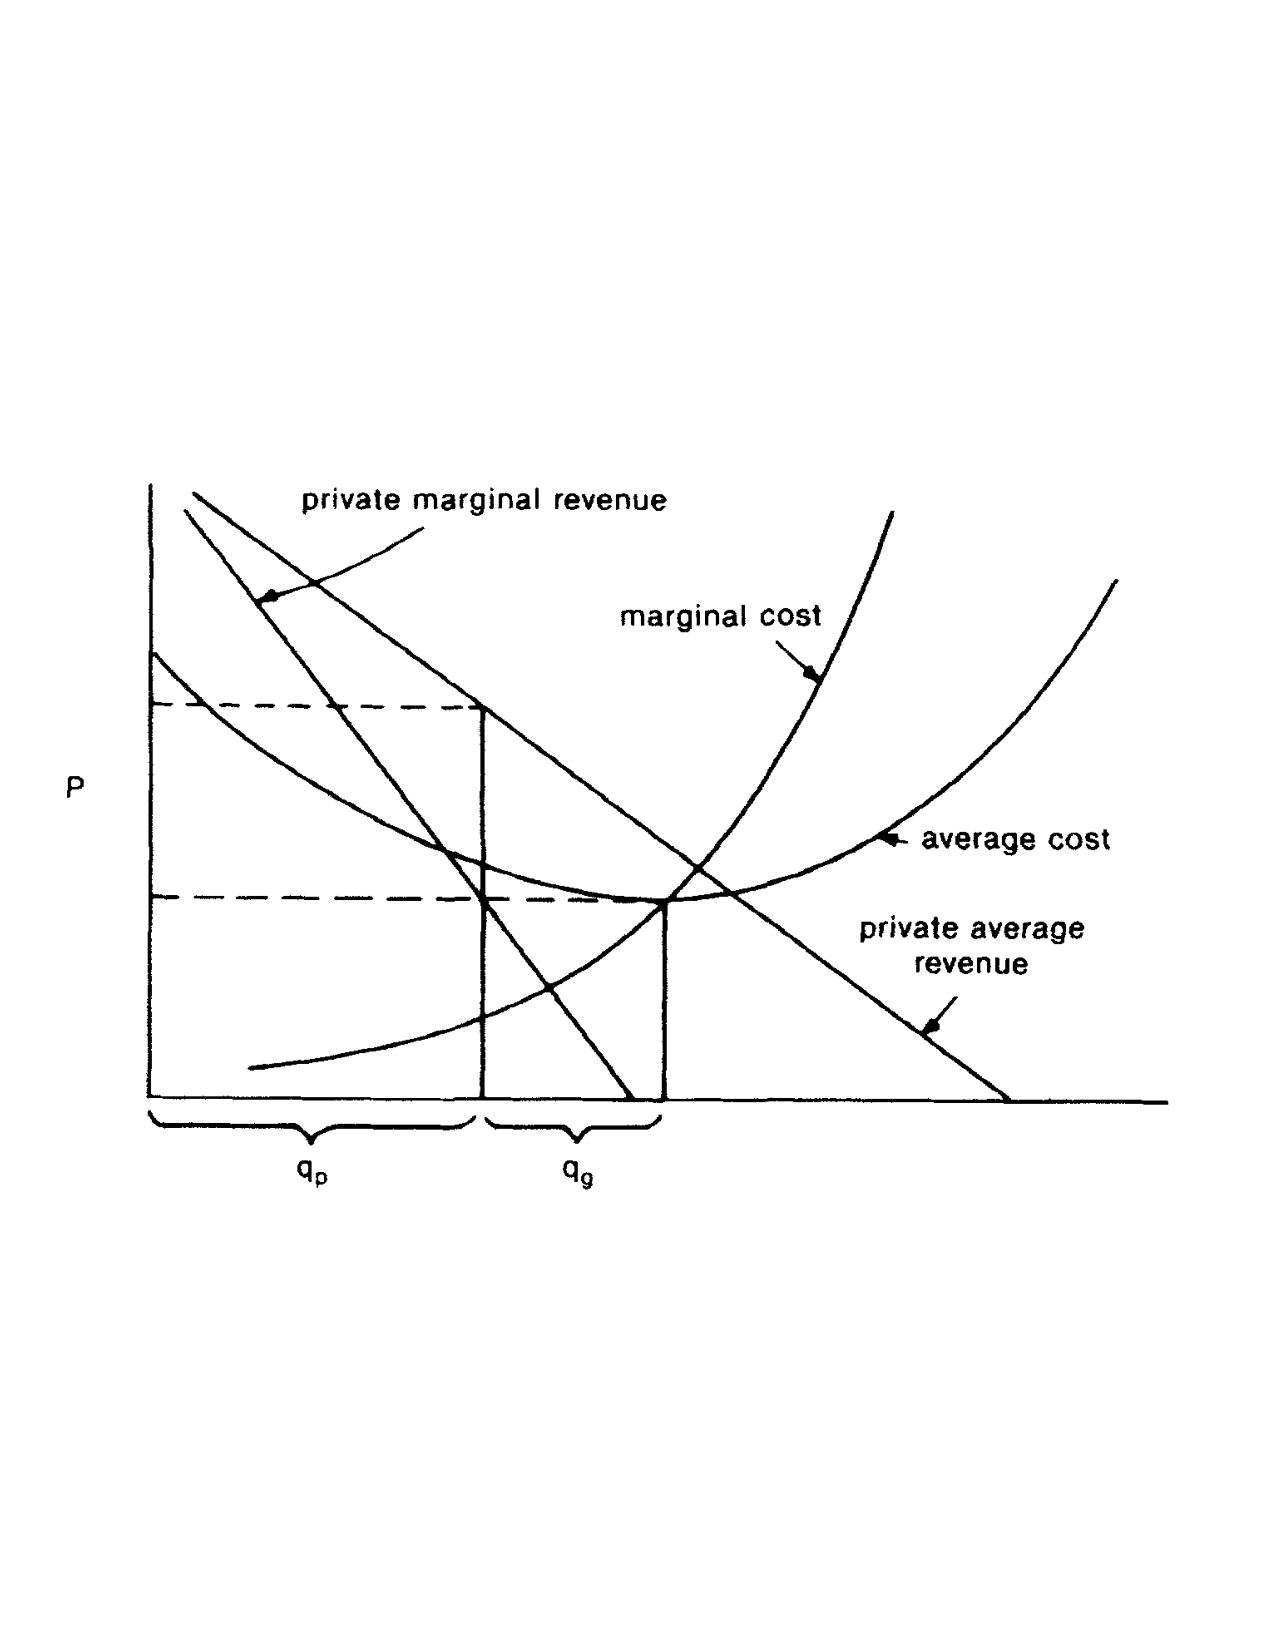
\includegraphics[scale=0.5]{hay}
\end{center}
\tiny Source: Hay (1983)
\end{frame}






%\begin{frame}
%\frametitle{Four Distinguishing Features of Hospital/Insurer Negotiations}
%\begin{enumerate}
%\item The set of hospitals with which an insurer negotiates is pre-determined by the health plan's provider network structure.
%\item Patients do not pay directly for the vast majority of their inpatient care.
%\item Health insurance choice is made by patients prior to the need for treatment.
%\item Hospitals negotiate over both inclusion in a network and reimbursement rates from treating the insurer's enrollees
%\end{enumerate}
%Structural bargaining models almost always condition on the network of the insurer and do not allow consumers to switch insurers in response to a network change.  GNT: 1st stage is negotiation over prices.  
%\end{frame}

\begin{frame}
\frametitle{Challenges for Standard Models}
Private prices are not directly set by hospitals.  
\begin{itemize}
\item Hospital/private insurer bargaining.
\item Procedure specific discounts in return for guaranteed referrals.
\item \textit{Relative} market power: $U^{\tau}V^{1-\tau}$?
\item Hospital Objective  Function?  
\end{itemize}
The effect of insurer competition on patient welfare is ambiguous:
\begin{itemize}
\item Insurer market power increases premiums
\item Insurer market power increases $\tau$, the relative bargaining power, which may imply lower hospital prices.  
\end{itemize} 
\end{frame}


\begin{frame}
\frametitle{Utility Maximizing Hospital}
\begin{displaymath}
 U\left( \pi_{j} = \sum_{i=1}^{N_{j}} \pi_{i,j}^{h} + \pi_{g,j}^{h}, \sum_{i=1}^{N_{j}} D_{i,j}^{h}, D_{g,j}^{h} \right),
\end{displaymath}
\begin{itemize}
\item $i=$ Insurer
\item $j=$ Hospital
\item $\pi_{j}=$ Total hopsital $j$ profit
\item $ \pi_{i,j}=$ Hospital $j$ from private insurer $i$
\item $ \pi_{g,j}=$ Hospital $j$ from the public payer.
\item $D_{i,j}=$ Hospital $j$ demand from insurer $i$.
\item $D_{i,j}=$ Hospital $j$ demand from the public sector.
\item[] $$\pi_{i,j}^{h}=D_{i,j}^{h}(p_{i,j}-c_{i}),$$
\begin{itemize}
\item $p_{i,j}=$ negotiated payment between insurer $i$ and hospital $j$
\end{itemize}
\end{itemize}
\end{frame}


\begin{frame}{Assumptions}
Assumptions:
\begin{itemize}
\item Patients are ``unaware or unable to determine their [financial] liability prior to choosing their provider.''
\item Average cost $=$ Marginal Cost $=$ constant.
\item Public payment is administratively set at $p_{g}$
\item Profits for insurer $i$ are:
\begin{equation}
\pi_{i}^{M} = D_{i} \left( \theta_{i} - \eta_{i} \right) - \sum_{j=1}^{N_{i}} D_{i,j}^{h} p_{i,j},
\label{eqn:ins_profit}
\end{equation}
\item $D_{i}=$ number of enrollees for insurer $i$
\item $\theta_{i}=$ insurer $i's$ premiums
\item $\eta_{i}=$ insurer $i'$ costs per-enrollee (other than inpatient hospital care), 
\item $D_{i,j}^{h} p_{i,j}=$ payments to hospitals for care provided to the insurer's enrollees.
\end{itemize}
\end{frame}



%\begin{itemize}
%\item Excess capacity
%\end{itemize}
%\item $U_{1}>0$, $U_{11}\leq 0$
%\item $U_{2}>0$, $U_{3}>0$ 
%\item $\pi_{2}<0$, $\pi_{11}<0$, $\pi_{12}\geq 0$
%\item $Q_{j}$, $P_{j}$ are exogenous

\begin{frame}{Negotiated Price}
The negotiated price between hospital $j$ and insurer $i$ is such that:
\begin{displaymath}
 p_{ij}= \arg \max_{p_{ij}} \left(\triangle U_{j} \right)^{b_{j}} \times \left(\triangle \pi^{M}_{i} \right)^{1-b_{j}},
 \label{eqn:neg_price}
\end{displaymath}
\begin{itemize}
\item $\triangle U_{j}=$ change in hospital $j$'s utility from reaching an agreement with insurer $i$
\item $\triangle \pi^{M}_{i}=$ the change in insurer $i's$ profits from an agreement with hospital $j$. 
\item $b_{j}=$ bargaining weight of hospital $j$ (expressed as the weight to which the hospital's payoffs are given in the overall net value.)
\end{itemize}
\end{frame}

%\begin{frame}{Relevant Comparative Static}
%\begin{displaymath}
%\deriv{p_{ij}}{p_{g}} = \frac{- b_{j} \triangle \pi_{i}^{M} \pderiv{^{2}U_{j}}{\pi_{j}^{2}}D_{g}^{h}}{D_{ij}^{h}\left(b_{j} D_{ij}^{h} \pderiv{^{2}U_{j}}{\pi_{j}^{2}} - (1-b_{j}) \pderiv{U_{j}}{\pi_{j}} \right)}.
%\end{displaymath}
%\end{frame}

\begin{frame}
\frametitle{Take Aways}
\begin{enumerate}
\item Hospital objective function matters.
\item Utility curvature in profits allows for cost-shifting.  
\item A utility maximizing hospital may cost shift depending on: 
\begin{itemize}
\item Relative market power
\item Market competition limits cost-shifting.
\end{itemize}
\item Financial shocks leave less room for nonprofits to pursue non-pecuninary goals.

\end{enumerate}
\end{frame}










\section{Extensions}
\subsection{Interesting Subgroups/ Models}


\begin{frame}
\frametitle{For-profit vs. Non-Profit Hospitals}
\begin{itemize}
%\item Differences between for-profits and non-profits (secular and religious) decrease in market competition and HMO penetration (Gruber, 1994; Cutler and Horwitz, 2000; Duggan, 2002; Kessler and McClellan, 2002; Horwitz and Nichols, 2007; Erus and Weisbrod, 2002)
%\begin{itemize}
%\item As market has grown more concentrated, perhaps more room for cost-shifting
%\end{itemize}
\item Non-profits constitute 2/3 of hospital beds (David, 2009)
\item Non-profits are charged with providing ``community benefits'' as a precondition for federal tax exemption:
\item Leading theories of nonprofit hospitals:
\begin{itemize}
\item For-profits in disguise.  Mixed evidence, nonprofits:
\begin{itemize}
\item Upcode less (Silverman and Skinner, 2003; Dafny, 2005
\item  Lower marginal cost but larger markups (Gaynor and Vogt, 2003)
\end{itemize}
\item Output maximizers
\item Social welfare maximizers
\item Perquisite maximizers
\end{itemize}
\item Chang and Jacobson (2010)
\end{itemize}
\end{frame}





\begin{frame}
\frametitle{Fixed Effects Regression Results: Nonprofit Only}
\begin{table}[htp]
\centering \normalsize
\caption{Non-profit Results}
\footnotesize
\begin{tabular}{llllll}
\hline	
\hline
 			& Log Mean				& Log Mean				& Medicaid 	   	& Medicare   		& Private  			\\
			& Payment		& Charge			& Discharges      		& Discharges       	& Discharges    \\
	\hline
\multicolumn{6}{c}{Non-profit Hospitals}\\											
\hline											
Net Penalty 	&	0.016***	&	0.007	&	-0.043*	&	-0.026***	&	-0.007	\\
	&	(0.005)	&	(0.009)	&	(0.024)	&	(0.007)	&	(0.012)	\\
\hline											
\multicolumn{6}{c}{Non-Profit Hospitals with Penalty Specific Trends} 											\\
						\hline					
Net Penalty 	&	0.013**	&	0.015	&	-0.037	&	-0.021***	&	-0.012	\\
	&	(0.005)	&	(0.009)	&	(0.026)	&	(0.007)	&	(0.013)	\\
p-value & 0.731 & 0.181 & 0.281 & 0.001 & 0.597 \\
\hline
\tiny Notes: $n=6,625$.  
\end{tabular}
\end{table}
\tiny Notes: All regressions include hospital and year fixed effects.  Further controls include those in our baseline specification for mean payments.  The p-values are in reference to the null hypothesis that trends in the outcome of interest are the same between ever-penalized and never-penalized hospitals conditional on the model covariates.  In cases in which independent variables are missing, we recode them and control for missing variable indicators to ensure a balanced panel.  Standard errors are clustered at the hospital level.  *** p-value$<$0.01, ** p-value$<$0.05, * p-value$<$0.1.
\end{frame}


\begin{frame}
\frametitle{Fixed Effects Regression Results: Nonprofit Only}
\begin{table}[htp]
\centering \normalsize
\caption{For-profit Results}
\footnotesize
\begin{tabular}{llllll}
\hline	
\hline
 			& Log Mean				& Log Mean				& Medicaid 	   	& Medicare   		& Private  			\\
			& Payment		& Charge			& Discharges      		& Discharges       	& Discharges    \\
	\hline
\multicolumn{6}{c}{For-profit Hospitals}\\											
\hline											
Net Penalty 	&	0.020	&	0.021	&	-0.018	&	-0.007	&	0.028	\\
	&	(0.014)	&	(0.021)	&	(0.050)	&	(0.017)	&	(0.019)	\\
\hline											
\multicolumn{6}{c}{For-Profit Hospitals with Penalty Specific Trends} 											\\
\hline											
Net Penalty	&	0.011	&	0.040*	&	0.001	&	-0.025	&	0.011	\\
	&	(0.014)	&	(0.023)	&	(0.049)	&	(0.016)	&	(0.019)	\\
p-value & 0.259 & 0.032 & 0.857 & 0.019 & 0.003 \\
\hline
\end{tabular}
\end{table}
\tiny Notes: All regressions include hospital and year fixed effects.  Further controls include those in our baseline specification for mean payments.  The p-values are in reference to the null hypothesis that trends in the outcome of interest are the same between ever-penalized and never-penalized hospitals conditional on the model covariates.  In cases in which independent variables are missing, we recode them and control for missing variable indicators to ensure a balanced panel.  Standard errors are clustered at the hospital level.  *** p-value$<$0.01, ** p-value$<$0.05, * p-value$<$0.1.
\end{frame}










\begin{frame}
\frametitle{Triple Difference by Payer Mix}
\begin{table}[htp]
\centering \normalsize
\caption{Payer Mix Results}
\footnotesize
\begin{tabular}{lll}
\hline	
 		& Log Mean & Log Mean   				 \\
		& Payment & Charge\\
\hline
Net Penalty	&	0.039***	&	0.042***	\\
	&	(0.010)	&	(0.012)	\\
\hspace{0.1in}* Public Share 2 	&	-0.020*	&	-0.013	\\
	&	(0.012)	&	(0.014)	\\
\hspace{0.1in}* Public Share 3	&	-0.032**	&	-0.043***	\\
	&	(0.013)	&	(0.015)	\\
\hspace{0.1in}* Public Share 4	&	-0.044***	&	-0.070***	\\
	&	(0.013)	&	(0.016)	\\
Public Share 2		&	0.006	&	0.047***	\\
	&	(0.010)	&	(0.013)	\\
Public Share 3		&	0.016	&	0.086***	\\
	&	(0.011)	&	(0.016)	\\
Public Share 4		&	0.023*	&	0.155***	\\
	&	(0.012)	&	(0.018)	\\
\hline
\end{tabular}
\end{table}
\tiny Notes: All regressions include hospital and year fixed effects.  Further controls include those in our baseline specification for mean payments.  The share of a hospital's patients insured by the public sector is broked into quartiles and interacted with penalty variables.  In cases in which independent variables are missing, we recode them and control for missing variable indicators to ensure a balanced panel.  Standard errors are clustered at the hospital level.  We restrict the sample to include at least 25 admissions per hospital per year.  *** p-value$<$0.01, ** p-value$<$0.05, * p-value$<$0.1.
\end{frame}


\begin{frame}
\frametitle{Payments vs. Charges: Hospital FE}
Cutler, McClellan, and Newhouse (2000).
\begin{table}[htp]
\centering \normalsize
\caption{Baseline Results}
\label{tab:samplemort}
\footnotesize
\begin{tabular}{llllll}
\hline	
 & Log Mean		& Log Mean		& Log Medicaid 	   	& Log Medicare   		& Log Private  			\\
	& Payment		& 	Charge		& Discharges      		& Discharges       		& Discharges        	\\
\hline
Net Penalty  	&	0.015***	&	0.008	&	-0.044**	&	-0.025***	&	-0.002	\\
	&	(0.005)	&	(0.008)	&	(0.021)	&	(0.006)	&	(0.010)	\\
\hline
\end{tabular}
\end{table}






\begin{table}[htp]
\centering \normalsize
\caption{Year Fixed Effects Only}
\footnotesize
\begin{tabular}{llllll}
\hline	
\hline
 			& Log Mean 		& Log Mean	& Medicaid 	   	& Medicare   		& Private  			\\
			& Payment		& 	Charge	& Discharges      	& Discharges       	& Discharges    \\
\hline											
Net Penalty	&	-0.061***	&	-0.053***	&	0.222***	&	0.097***	&	0.070***	\\
	&	(0.015)	&	(0.018)	&	(0.044)	&	(0.025)	&	(0.022)	\\
\end{tabular}
\end{table}
\tiny Notes: Further controls include those in our baseline specification for mean payments.  The p-value in the first row of results is in reference to the null hypothesis that trends in the outcome of interest are the same between ever-penalized and never-penalized hospitals conditional on the model covariates.  In cases in which independent variables are missing, we recode them and control for missing variable indicators to ensure a balanced panel.  Standard errors are clustered at the hospital level.  *** p-value$<$0.01, ** p-value$<$0.05, * p-value$<$0.1.
\end{frame}

\begin{frame}
\frametitle{Changes in Quality}
\begin{table}[htp]
\centering \normalsize
\caption{Profit Index}
\label{tab:samplemort}
\footnotesize
\begin{tabular}{llll}
\hline\hline
 & Profit Index & Average DRG & Average LOS \\
 & 			& Weight & \\
\hline							
Net Penalty  		&	0.002	&	0.004	&	0.015	\\
	&	(0.001)	&	(0.004)	&	(0.012)	\\
\hline
\tiny Notes: $n=8,316$.  
\end{tabular}
\end{table}
\tiny All regressions include hospital and year fixed effects and other hospital level controls include bed count and labor force.  Market power variables are constructed as the overall county market share tercile.  Large market is a binary variable for a hospital in the top half of the market size distribution.  In cases in which independent variables are missing, we recode them and control for missing variable indicators to ensure a balanced panel.  Standard errors are clustered at the hospital level.  *** p-value$<$0.01, ** p-value$<$0.05, * p-value$<$0.1.
\end{frame}




\begin{frame}
\frametitle{Condition Specific Payment Effects}
\begin{table}[htp]
\centering \normalsize
\caption{Payments for Condition Specific Admissions}
\scriptsize
\begin{tabular}{ccccccc}
\hline	
\hline
 							& Nervous  	& Respiratory  	 & Circulatory    & Musculoskeletal   		& Labor and & Neonatal \\
							&  System		&  System      	&  System     	&  System        		& Delivery   &	\\
\hline
Net Penalty 					& 0.022***		&	0.000 	&	0.022***	&	0.004	&	-0.001	&	0.015	\\
							& (0.010)		&	(0.011)	&	(0.008)	&	(0.007)	&	(0.005)	&	(0.010)	\\
\hline
n							& 1,410		&	1,770 	&	2,754  	&	3,084   	&	5,232	&	3,198	\\
Mean 						&13,878.62	&	11,984.62	&	13,222.00	&	13,088.46	&	11,507.31	&	9,038.22	\\
\hline
\end{tabular}
\end{table}
\tiny Notes: All regressions include hospital and year fixed effects.  The dependent variable is the log of average payments for each condition.  Further controls include those in our baseline specification for mean payments.  The dependent variable in each column is the log of the payment for the associated acute care admission.  In cases in which independent variables are missing, we recode them and control for missing variable indicators to ensure a balanced panel.  Standard errors are clustered at the hospital level.  We restrict the sample to include at least 25 admissions per hospital per year.  *** p-value$<$0.01, ** p-value$<$0.05, * p-value$<$0.1.
\end{frame}


\section{Discussion and Next Steps}
\subsection{Discussion and Next Steps}
\begin{frame}
\frametitle{Larger Trends}
\begin{itemize}
\item Health Consumption Expenditures at Hospitals remain approximately 1/3 of total National Health Expenditures.
\item  Starting this year (FY 2017), HRRP has added coronary artery bypass graft (CABG) surgery: $\$$130,000 per procedure, wide variance, continued care.
 \end{itemize}
\end{frame}

\begin{frame}
\frametitle{Hospital Concentration}
\begin{center}
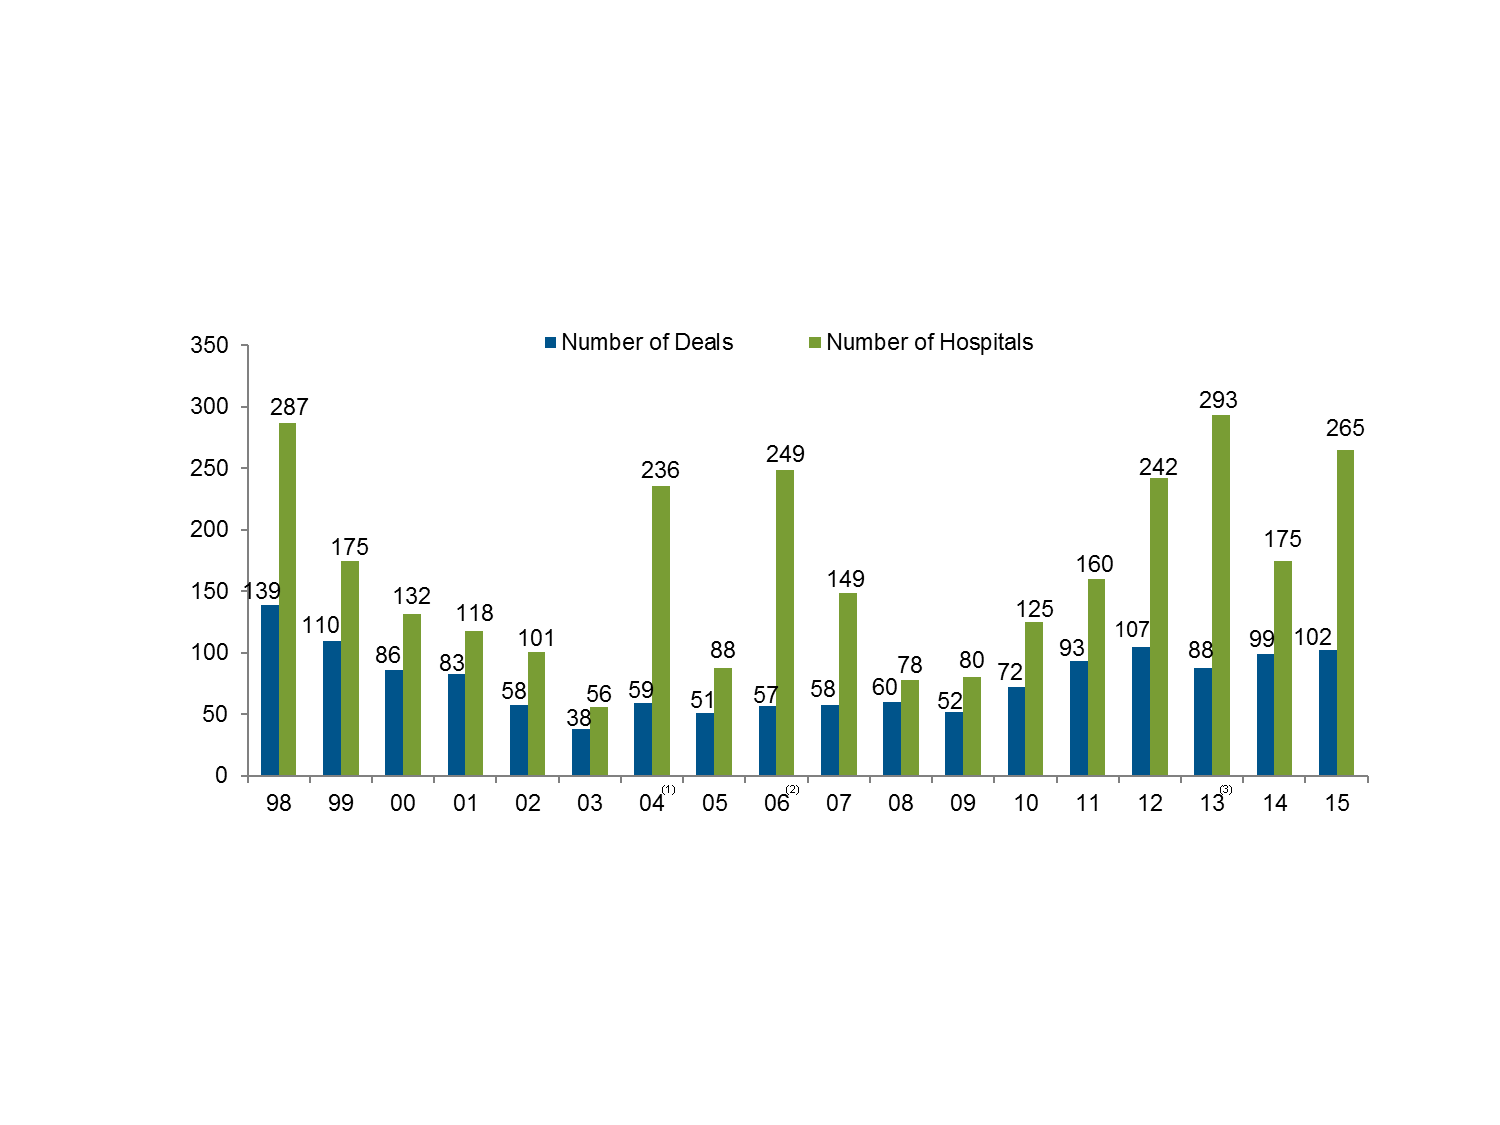
\includegraphics[scale=0.5]{chart29}
\end{center}
\tiny Source: AHA Trendwatch Chartbook 2016.  
\end{frame}

\begin{frame}
\frametitle{Hospital Concentration}
\begin{center}
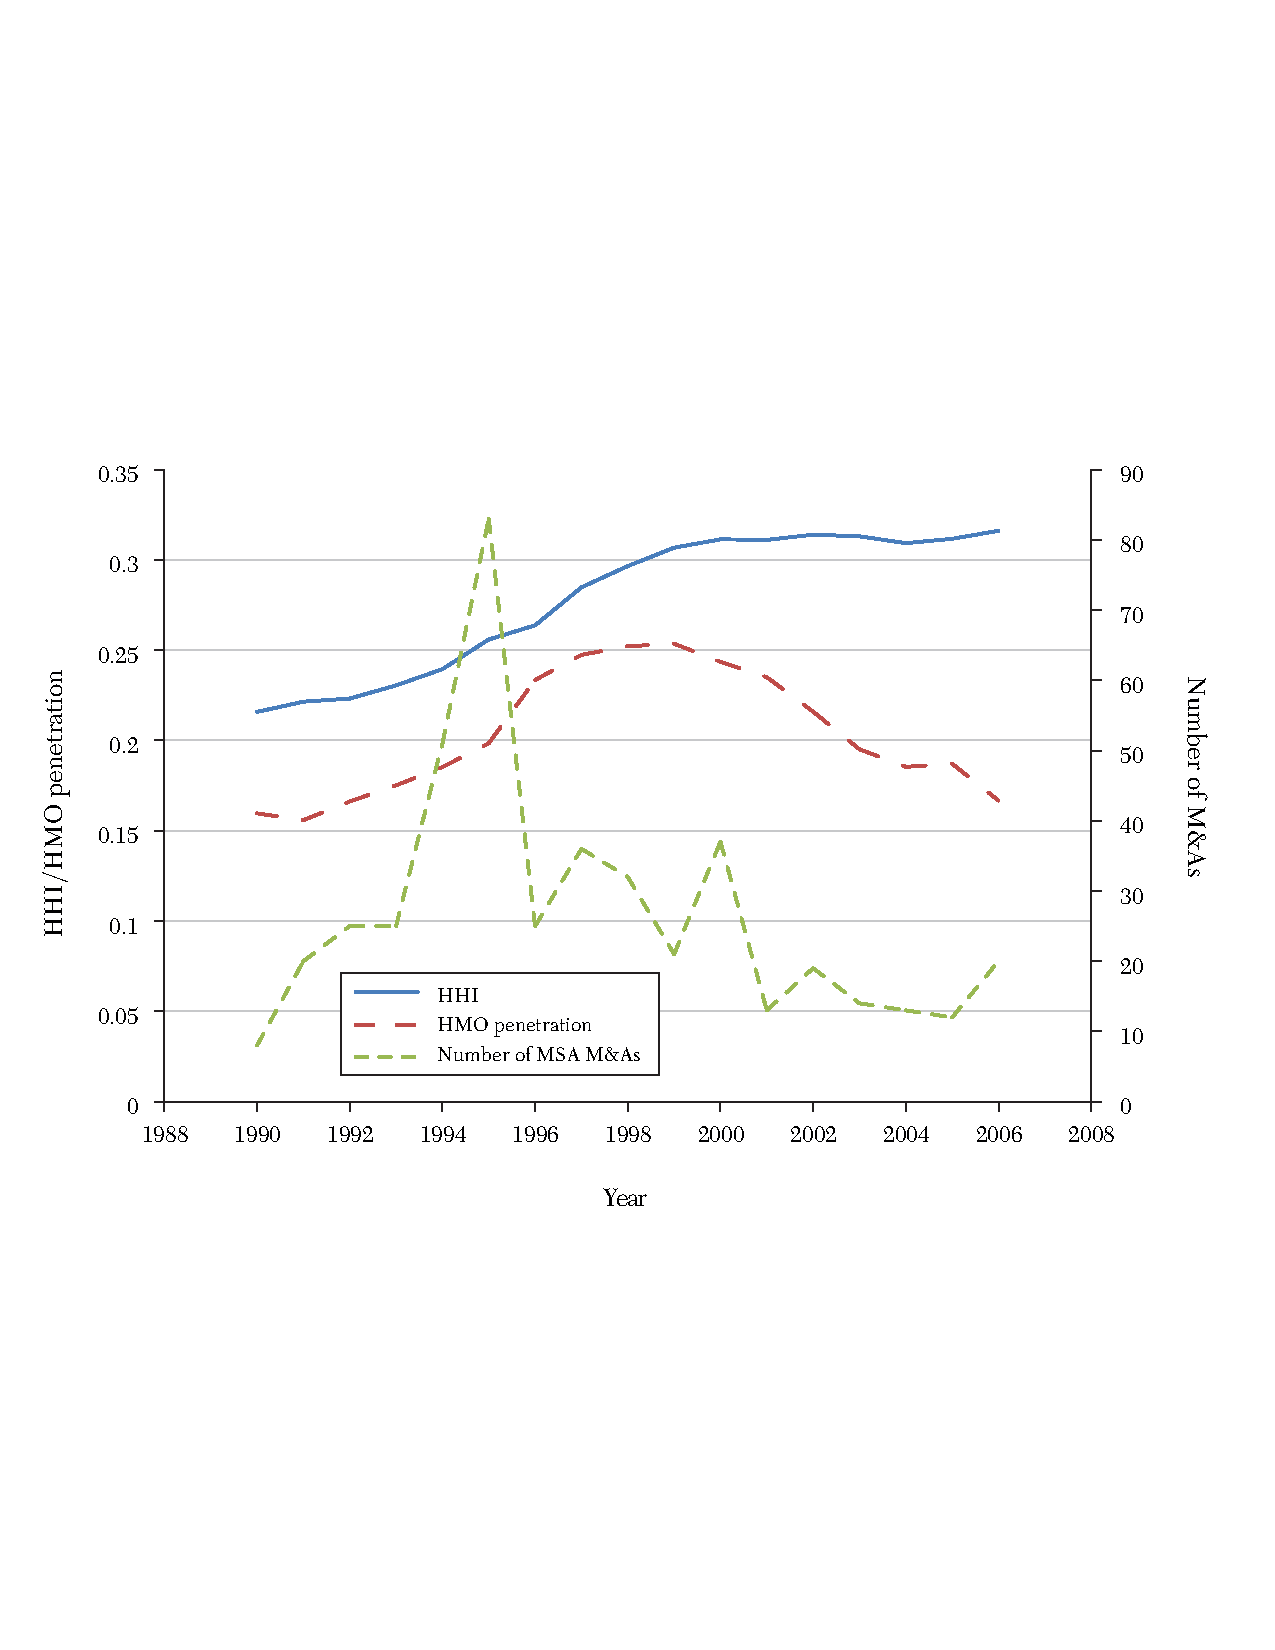
\includegraphics[scale=0.5]{gay1}
\end{center}
\tiny Source: Gaynor, Ho, and Town (2015)
\end{frame}

\begin{frame}
\frametitle{Hospital Concentration}
\begin{center}
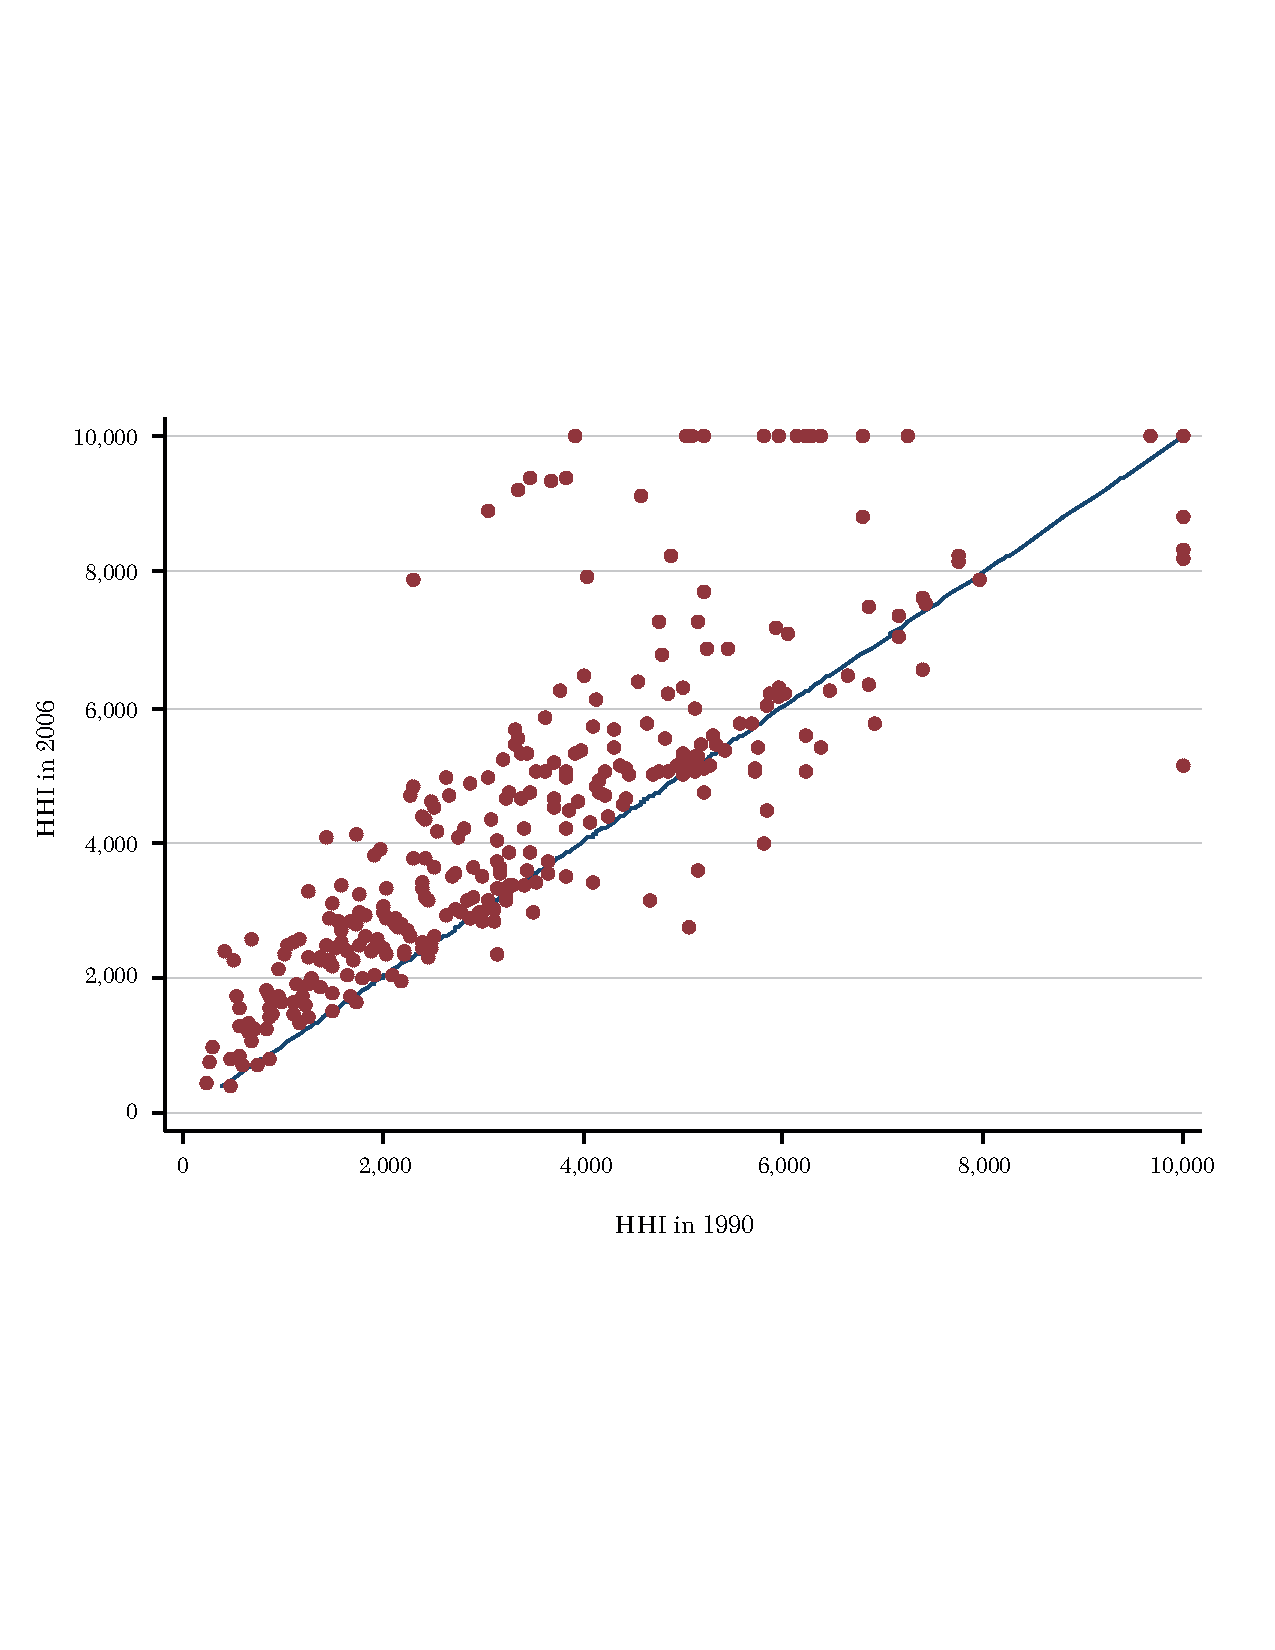
\includegraphics[scale=0.5]{gay2}
\end{center}
\tiny Source: Gaynor, Ho, and Town (2015)
\end{frame}



\begin{frame}
\frametitle{Conclusion}
\begin{itemize}
\item We leverage unique data and plausibly exogenous variation in public reimbursement to study cost-shifting in hospitals.
\item Evidence suggests that non-profit hospitals may increase prices following reimbursement cuts.  
\item $\$$0.50 to the dollar.  Concentrated in 
\begin{itemize}
\item Hospitals with large private patient shares
\item Non-Profits (Statistically)
\end{itemize}
\end{itemize}
\end{frame}

\begin{frame}
\huge
Thank You!
\begin{itemize}
\item Comments to: darden@gwu.edu
\item medarden.com
\end{itemize}
\end{frame}




\end{document}

